%\documentclass[hyperref={pdfpagelabels=false},slidetop,9pt]{beamer}
\documentclass[slidetop,8pt]{beamer}
\usepackage[T1]{fontenc}
\usepackage[utf8]{inputenc}
\newcommand{\nom}{Porte conteneur}
\newcommand{\sequence}{03}
\newcommand{\num}{04}
\newcommand{\type}{TD}
\newcommand{\descrip}{Résolution d'un problème en utilisant des méthodes algorithmiques}
\newcommand{\competences}{Alt-C3: Concevoir un algorithme répondant à un problème précisément posé}
\usepackage{etex}
\usepackage{tikz}
\usepackage[european]{circuitikz}
\usepackage{pgf}
\usepackage[all]{xy}
\usepackage{pgfpages}
\usepackage{graphbox}
\usepackage{pdfpages}
\usepackage[adobe-utopia]{mathdesign}
\usepackage{ifthen}
\usepackage{cancel}
\usepackage{framed}
\usepackage{subfig}
\usepackage{tabularx}
\usepackage{setspace}
\usepackage{soul}
\usepackage{schemabloc}
\usepackage{eqnarray}
\usepackage[dot, phantomtext]{dashundergaps}
\usepackage{media9}
\usepackage{multimedia}

\author{Renaud Costadoat}
\institute{Lycée Dorian}

\usepackage{multido}
\usepackage{multirow}
\usepackage{multicol} % Portions de texte en colonnes
\usepackage{flafter}%floatants après la référence

\usepackage{color}
\usepackage{xcolor}
\usepackage{colortbl}

\usepackage[gen]{eurosym}
\usepackage{tikz}
%\usepackage{pstricks,pst-node,pst-tree,pst-solides3d}
\usepackage{lmodern}
\usepackage[francais]{babel}
\usepackage{pslatex}
\usetheme{renaud}
\usepackage{times}
\usepackage{amsmath}
\usepackage{verbatim}
\usepackage{moreverb}
%\usetikzlibrary{arrows,shapes}
\usepackage{graphicx}
\usepackage{psfrag}
\usepackage{wrapfig}
\usepackage{etoolbox}

\definecolor{gris25}{gray}{0.75}
\definecolor{bleu}{RGB}{18,33,98}
\definecolor{bleuf}{RGB}{42,94,171}
\definecolor{bleuc}{RGB}{231,239,247}
\definecolor{rougef}{RGB}{185,18,27}
\definecolor{rougec}{RGB}{255,188,204}%255,230,231
\definecolor{vertf}{RGB}{103,126,82}
\definecolor{vertc}{RGB}{220,255,191}

\setlength\parindent{24pt}
\parskip 7.2pt
\parindent 8pt

\newenvironment{rem}[1][\hsize]%
{%
    \def\FrameCommand
   {%
\rotatebox{90}{\textit{\textsf{Remarque}}} 
       {\color{bleuf}\vrule width 3pt}%
       \hspace{0pt}%must no space.
       \fboxsep=\FrameSep\colorbox{bleuc}%
  }%
    \MakeFramed{\hsize#1\advance\hsize-\width\FrameRestore}%
}%
{\endMakeFramed}%


\newenvironment{savoir}[1][\hsize]%
{%
    \def\FrameCommand
    {%
\rotatebox{90}{\textit{\textsf{Savoir}}} 
        {\color{bleuf}\vrule width 3pt}%
        \hspace{0pt}%must no space.
        \fboxsep=\FrameSep\colorbox{bleuc}%
    }%
    \MakeFramed{\hsize#1\advance\hsize-\width\FrameRestore}%
}%
{\endMakeFramed}%

\newenvironment{prob}[1][\hsize]%
{%
    \def\FrameCommand%
    {%
\rotatebox{90}{\textit{\textsf{Problématique}}} 
        {\color{rougef}\vrule width 3pt}%
        \hspace{0pt}%must no space.
        \fboxsep=\FrameSep\colorbox{rougec}%
    }%
    \MakeFramed{\hsize#1\advance\hsize-\width\FrameRestore}%
}%
{\endMakeFramed}%

\newenvironment{obj}[1][\hsize]%
{%
    \def\FrameCommand%
    {%
\rotatebox{90}{\textit{\textsf{Objectif}}} 
        {\color{vertf}\vrule width 3pt}%
        \hspace{0pt}%must no space.
        \fboxsep=\FrameSep\colorbox{vertc}%
    }%
    \MakeFramed{\hsize#1\advance\hsize-\width\FrameRestore}%
}%
{\endMakeFramed}%

\newenvironment{defi}[1][\hsize]%
{%
    \def\FrameCommand%
    {%
\rotatebox{90}{\textit{\textsf{Definition}}} 
        {\color{bleuf}\vrule width 3pt}%
        \hspace{0pt}%must no space.
        \fboxsep=\FrameSep\colorbox{rougec}%
    }%
    \MakeFramed{\hsize#1\advance\hsize-\width\FrameRestore}%
}%
{\endMakeFramed}%


\newenvironment{hypo}[1][\hsize]%
{%
    \def\FrameCommand%
    {%
\rotatebox{90}{\textit{\textsf{Hypothèse\\}}} 
        {\color{bleuf}\vrule width 3pt}%
        \hspace{0pt}%must no space.
        \fboxsep=\FrameSep\colorbox{bleuc}%
    }%
    \MakeFramed{\hsize#1\advance\hsize-\width\FrameRestore}%
}%
{\endMakeFramed}%


\newenvironment{prop}[1][\hsize]%
{%
    \def\FrameCommand%
    {%
\rotatebox{90}{\textit{\textsf{Propriété}}} 
        {\color{bleuf}\vrule width 3pt}%
        \hspace{0pt}%must no space.
        \fboxsep=\FrameSep\colorbox{bleuc}%
    }%
    \MakeFramed{\hsize#1\advance\hsize-\width\FrameRestore}%
}%
{\endMakeFramed}%

\newenvironment{props}[1][\hsize]%
{%
    \def\FrameCommand%
    {%
\rotatebox{90}{\textit{\textsf{Propriétés}}} 
        {\color{bleuf}\vrule width 3pt}%
        \hspace{0pt}%must no space.
        \fboxsep=\FrameSep\colorbox{bleuc}%
    }%
    \MakeFramed{\hsize#1\advance\hsize-\width\FrameRestore}%
}%
{\endMakeFramed}%

\newenvironment{exemple}[1][\hsize]%
{%
    \def\FrameCommand%
    {%
\rotatebox{90}{\textit{\textsf{Exemple}}} 
        {\color{vertf}\vrule width 3pt}%
        \hspace{0pt}%must no space.
        \fboxsep=\FrameSep\colorbox{vertc}%
    }%
    \MakeFramed{\hsize#1\advance\hsize-\width\FrameRestore}%
}%
{\endMakeFramed}%

\newenvironment{resultat}[1][\hsize]%
{%
    \def\FrameCommand%
    {%
\rotatebox{90}{\textit{\textsf{Resultat}}} 
        {\color{rougef}\vrule width 3pt}%
%        {\color{bleuf}\vrule width 3pt}%
        \hspace{0pt}%must no space.
        \fboxsep=\FrameSep\colorbox{rougec}%
    }%
    \MakeFramed{\hsize#1\advance\hsize-\width\FrameRestore}%
}%
{\endMakeFramed}%

\newenvironment{methode}[1][\hsize]%
{%
    \def\FrameCommand%
    {%
\rotatebox{90}{\textit{\textsf{Méthode\\}}} 
        {\color{rougef}\vrule width 3pt}%
        \hspace{0pt}%must no space.
        \fboxsep=\FrameSep\colorbox{rougec}%
    }%
    \MakeFramed{\hsize#1\advance\hsize-\width\FrameRestore}%
}%
{\endMakeFramed}%

\newenvironment{theo}[1][\hsize]%
{%
    \def\FrameCommand%
    {%
\rotatebox{90}{\textit{\textsf{Théorème\\}}} 
        {\color{rougef}\vrule width 3pt}%
        \hspace{0pt}%must no space.
        \fboxsep=\FrameSep\colorbox{rougec}%
    }%
    \MakeFramed{\hsize#1\advance\hsize-\width\FrameRestore}%
}%
{\endMakeFramed}%

\newenvironment{warn}[1][\hsize]%
{%
    \def\FrameCommand%
    {%
\rotatebox{90}{\textit{\textsf{Attention\\}}} 
        {\color{rougef}\vrule width 3pt}%
        \hspace{0pt}%must no space.
        \fboxsep=\FrameSep\colorbox{rougec}%
    }%
    \MakeFramed{\hsize#1\advance\hsize-\width\FrameRestore}%
}%
{\endMakeFramed}%

% \usepackage{pstricks}
%\usepackage{minitoc}
% \setcounter{minitocdepth}{4}

\setcounter{tocdepth}{2}

% \mtcselectlanguage{french} 

%\usepackage{draftcopy}% "Brouillon"
% \usepackage{floatflt}
\usepackage{psfrag}
%\usepackage{listings} % Permet d'insérer du code de programmation
\renewcommand{\baselinestretch}{1.2}

% Changer la numérotation des figures :
% ------------------------------------
% \makeatletter
% \renewcommand{\thefigure}{\ifnum \c@section>\z@ \thesection.\fi
%  \@arabic\c@figure}
% \@addtoreset{figure}{section}
% \makeatother
 


%%%%%%%%%%%%
% Définition des vecteurs %
%%%%%%%%%%%%
 \newcommand{\vect}[1]{\overrightarrow{#1}}

%%%%%%%%%%%%
% Définition des torseusr %
%%%%%%%%%%%%

 \newcommand{\torseur}[1]{%
\left\{{#1}\right\}
}

\newcommand{\torseurcin}[3]{%
\left\{\mathcal{#1} \left(#2/#3 \right) \right\}
}

\newcommand{\torseurstat}[3]{%
\left\{\mathcal{#1} \left(#2\rightarrow #3 \right) \right\}
}

 \newcommand{\torseurc}[8]{%
%\left\{#1 \right\}=
\left\{
{#1}
\right\}
 = 
\left\{%
\begin{array}{cc}%
{#2} & {#5}\\%
{#3} & {#6}\\%
{#4} & {#7}\\%
\end{array}%
\right\}_{#8}%
}

 \newcommand{\torseurcol}[7]{
\left\{%
\begin{array}{cc}%
{#1} & {#4}\\%
{#2} & {#5}\\%
{#3} & {#6}\\%
\end{array}%
\right\}_{#7}%
}

 \newcommand{\torseurl}[3]{%
%\left\{\mathcal{#1}\right\}_{#2}=%
\left\{%
\begin{array}{l}%
{#1} \\%
{#2} %
\end{array}%
\right\}_{#3}%
}

 \newcommand{\vectv}[3]{%
\vect{V\left( {#1} \in {#2}/{#3}\right)}
}


\newcommand{\vectf}[2]{%
\vect{R\left( {#1} \rightarrow {#2}\right)}
}

\newcommand{\vectm}[3]{%
\vect{\mathcal{M}\left( {#1}, {#2} \rightarrow {#3}\right)}
}


 \newcommand{\vectg}[3]{%
\vect{\Gamma \left( {#1} \in {#2}/{#3}\right)}
}

 \newcommand{\vecto}[2]{%
\vect{\Omega\left( {#1}/{#2}\right)}
}

\newcommand{\reponse}[1][4]
{
\multido{}{#1}
{
\begin{center}
\makebox[0.9\linewidth]{\dotfill} \end{center}
}}


% }$$\left\{\mathcal{#1} \right\}_{#2} =%
% \left\{%
% \begin{array}{c}%
%  #3 \\%
%  #4 %
% \end{array}%
% \right\}_{#5}}


%  ------------------------------------------
% | Modification du formatage des sections : | 
%  ------------------------------------------

% Grands titres :
% ---------------

\newcommand{\titre}[1]{%
\begin{center}
      \bigskip
      \rule{\textwidth}{1pt}
      \par\vspace{0.1cm}
      
      \textbf{\large #1}
      \par\rule{\textwidth}{1pt}
    \end{center}
    \bigskip
  }

% Supprime le numéro du chapitre dans la numérotation des sections:
% -----------------------------------------------------------------
\makeatletter
\renewcommand{\thesection}{\@arabic\c@section}
\makeatother


% \titleformat{\chapter}[display]
% {\normalfont\Large\filcenter}
% {}
% {1pc}
% {\titlerule[1pt]
%   \vspace{1pc}%
%   \Huge}[\vspace{1ex}%
% \titlerule]


%%%% Chapitres Comme PY Pechard %%%%%%%%%
% numéro du chapitre
\DeclareFixedFont{\chapnumfont}{OT1}{phv}{b}{n}{80pt}
% pour le mot « Chapitre »
\DeclareFixedFont{\chapchapfont}{OT1}{phv}{m}{it}{40pt}
% pour le titre
\DeclareFixedFont{\chaptitfont}{T1}{phv}{b}{n}{25pt}

\definecolor{gris}{gray}{0.75}
\setbeamertemplate{section in toc}[sections numbered]

\newlength{\RoundedBoxWidth}
\newsavebox{\GrayRoundedBox}
\newenvironment{GrayBox}[1][\dimexpr\textwidth-4.5ex]%
   {\setlength{\RoundedBoxWidth}{\dimexpr#1}
    \begin{lrbox}{\GrayRoundedBox}
       \begin{minipage}{\RoundedBoxWidth}}%
   {   \end{minipage}
    \end{lrbox}
    \begin{center}
    \begin{tikzpicture}%
       \draw node[draw=bleuf,fill=bleuc,rounded corners,%
             inner sep=2ex,text width=\RoundedBoxWidth]%
             {\usebox{\GrayRoundedBox}};
    \end{tikzpicture}
    \end{center}}
    
\ifdef{\prive}{\pgfpagesuselayout{2 on 1}[a4paper,border shrink=0mm]}
\ifdef{\prive}{\setbeamertemplate{navigation symbols}{}}
\setbeamertemplate{itemize item}[ball]
%\setbeamertemplate{blocks}[rounded]%[shadow=true]
\setbeamercolor{block title}{fg=white,bg=grisf}        % titre block normal 
\setbeamercolor{block body}{fg=grisf,bg=grisc!50}      % corps block normal
\setbeamercolor{block body alerted}{fg=white,bg=warning}   % idem pour un block alerte

\title{\nom}
\date{S\sequence \ - \type\num}

\begin{document}
\shorthandoff{:!}
\bibliographystyle{abbrvnat-fr}

\usebackgroundtemplate%
{%
    \centering
\includegraphics[width=\paperwidth]{../../img/fond2}%
}

{
\setbeamertemplate{navigation symbols}{}
\setbeamertemplate{headline}[pagetitre]
\setbeamertemplate{footline}[pagetitre]
\usebackgroundtemplate{\centering
\includegraphics[width=\paperwidth]{../../img/fond}}
\frame{\titlepage}
}



\section{Présentation} 

\begin{frame}[fragile]
\frametitle{Introduction}

\begin{wrapfigure}[15]{r}{0.3\textwidth}
\vspace{-0.5cm}
  \begin{center}
    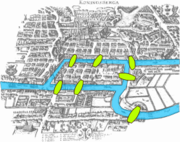
\includegraphics[width=0.9\linewidth]{img/Konigsberg_bridges}
  \end{center}
  \caption{Ponts de \textit{Königsberg}}
\end{wrapfigure}

La théorie des graphes un domaine très important en informatique et dans les sciences en général. L'origine des graphes remonte au problème de Königsberg étudié par Euler en 1736.

La ville de \textit{Königsberg} est construite autour de deux îles situées sur le fleuve \textit{Pregel} et reliées entre elles par un pont.

6 autres ponts relient les rives de la rivière à l'une ou l'autre des deux îles.

Le problème que s'est posée Euler consiste à déterminer
 s'il existe ou non une promenade dans les rues de Königsberg permettant, à partir d'un point de départ au choix, de passer une et une seule fois par chaque pont, et de revenir à son point de départ, étant entendu qu'on ne peut traverser le fleuve qu'en passant sur les ponts.
\end{frame}

\begin{frame}[fragile]
\frametitle{Définitions}

\vspace{0.5cm}

\begin{defi}
Un \textbf{graphe} $G = (S,A)$ est un couple composé :
\begin{itemize}
\item d'un ensemble $S$ de points appelés \textbf{sommets} (ou vertex en anglais),
\item d'un ensemble $A$ de liens appelés \textbf{arêtes} (ou edge en anglais).
\end{itemize} 
\end{defi}

\begin{minipage}[l]{0.4\linewidth}
\begin{center}
\begin{tikzpicture}[scale=0.8]
\tikzstyle{sommet}=[circle,draw,fill=gray!20]
\draw (90:1) node[sommet]{0}
-- (162:1) node[sommet]{1}
-- (234:1) node[sommet]{2}
-- (306:1) node[sommet]{3}
-- (378:1) node[sommet]{4}
-- cycle;
\end{tikzpicture}
\end{center}
\end{minipage}
\begin{minipage}[l]{0.4\linewidth}
Ce graphe $G=(S,A)$ est défini par :
\begin{itemize}
\item $S={0,1,2,3,4}$
\item $A={'01','12','23','24','40'}$
\end{itemize}
\medskip
\end{minipage}

\begin{itemize}
 \item Les sommets reliés par une arête sont ses \textbf{extrémités},
 \item Une arête forme une \textbf{boucle} si ces extrémités sont identiques,
 \item Les sommets sont \textbf{voisins} s’ils sont reliés par une arête,
 \item Les arêtes peuvent être \textbf{orientées} (\textit{flèches}) et donc imposer un sens de parcours des sommets.
\end{itemize}
\end{frame}

\begin{frame}[fragile]
\frametitle{Définitions}

Un graphe est dit \textbf{planaire} s'il existe une représentation dans laquelle aucune de ces arêtes ne se croisent.
\begin{center}
\begin{tikzpicture}[scale=0.5]
\tikzstyle{sommet}=[circle,draw,fill=gray!20]
\draw (1,-2) node[above] {Graphe planaire} ;
\node[sommet] (A0) at (0.3,1) {0};
\node[sommet] (A1) at (-1,1) {1};
\node[sommet] (A2) at (1,2) {2};
\node[sommet] (A3) at (1,0) {3};
\node[sommet] (A4) at (3,1) {4};
\tikzstyle{sommet}=[circle,draw,fill=gray!20]
\draw (7,-2) node[above] {Graphe planaire} ;
\node[sommet] (B0) at (7.7,1) {0};
\node[sommet] (B1) at (5,1) {1};
\node[sommet] (B2) at (7,2) {2};
\node[sommet] (B3) at (7,0) {3};
\node[sommet] (B4) at (9,1) {4};
\draw (13,-2) node[above] {Graphe \textbf{non} planaire} ;
\node[sommet] (C0) at (12.25,2.299) {0};
\node[sommet] (C1) at (11.5,1)     {1};
\node[sommet] (C2) at (12.25,-0.299) {2};
\node[sommet] (C3) at (13.75,-0.299) {3};
\node[sommet] (C4) at (14.5,1)     {4};
\node[sommet] (C5) at (13.75,2.299) {5};
\draw (A0) -- (A1) -- (A2) -- (A3)-- (A1) ;
\draw (A2) -- (A4) -- (A3) ;
\draw (B0) -- (B1) -- (B2) -- (B3)-- (B1) ;
\draw (B2) -- (B4) -- (B3) ;
\draw (C0) -- (C1) -- (C2) -- (C3)-- (C4)-- (C5)--(C0) ;
\draw (C4) -- (C1) -- (C3) -- (C5) -- (C1);
\draw (C0) -- (C2) -- (C4) -- (C0)-- (C3);
\end{tikzpicture}
\end{center}

Un graphe est dit \textbf{simple} si au plus une arête relie deux sommets et s'il n'y a pas de \textbf{boucle} sur un sommet. Sinon, c'est un \textbf{multigraphe}.

\begin{center}
\begin{tikzpicture}[scale=0.5]
\tikzstyle{sommet}=[circle,draw,fill=gray!20]
\draw (1.5,-1.5) node[above] {Graphe simple} ;
\node[sommet] (A0) at (0,0) {0};
\node[sommet] (A1) at (0,2) {1};
\node[sommet] (A2) at (2,2) {2};
\node[sommet] (A3) at (2,0) {3};
\node[sommet] (A4) at (3,1) {4};
\draw (11.5,-1.5) node[above] {Multigraphe} ;
\node[sommet] (B0) at (10,0) {0};
\node[sommet] (B1) at (10,2) {1};
\node[sommet] (B2) at (12,2) {2};
\node[sommet] (B3) at (12,0) {3};
\node[sommet] (B4) at (13,1) {4};
\draw (A0) -- (A1) -- (A2) -- (A0) ;
\draw (A2) -- (A4) -- (A3) -- (A0) ;
\draw (B0) to[bend right] (B1);
\draw (B0) to[bend left] (B1);
\draw (B4) to[out=45,in=90] (14,1) to[out=-90,in=-45] (B4);
\draw (B1) -- (B2) -- (B3) -- (B4) -- (B2) -- (B0) -- (B3) ;
\end{tikzpicture}
\end{center}
\end{frame}

\begin{frame}[fragile]
\frametitle{Définitions}

Un graphe est \textbf{connexe} s’il est possible, à partie de n’importe quel sommet de rejoindre tous les autres sommets en suivant les arêtes. Un graphe non connexe se décompose en plusieurs sous graphes connexes. Un graphe est \textbf{complet} si tous les sommets sont des voisins directs.

\begin{center}
\begin{tikzpicture}[scale=0.5]
\tikzstyle{sommet}=[circle,draw,fill=gray!20]
\draw (1.5,-1.5) node[above] {Graphe non connexe} ;
\node[sommet] (A0) at (0,0) {0};
\node[sommet] (A1) at (0,2) {1};
\node[sommet] (A2) at (2,2) {2};
\node[sommet] (A3) at (2,0) {3};
\node[sommet] (A4) at (3,1) {4};
\draw (11.5,-1.5) node[above] {Graphe complet} ;
\node[sommet] (B0) at (10,0) {0};
\node[sommet] (B1) at (10,2) {1};
\node[sommet] (B2) at (12,2) {2};
\node[sommet] (B3) at (12,0) {3};
\node[sommet] (B4) at (13,1) {4};
\draw (A0) -- (A1) -- (A2) --(A0) ;
\draw (A4) -- (A3) ;
\draw (B0) -- (B1) -- (B2) -- (B3) -- (B4) -- (B0) -- (B2) -- (B4) -- (B1) -- (B3) -- (B0);
\end{tikzpicture}
\end{center}
\vspace{-0.5cm}
Un graphe est dit \textbf{biparti} si son ensemble de sommets $S$ peut être partitionné en deux sous ensembles de sommets $A$ et $B$ de façon à ce que toute arrête ait une extrémité dans $A$ et une extrémité dans $B$. Une \textbf{étoile} est donc un graphe biparti dont l'une des bipartitions n'a qu'un sommet. 

\vspace{-0.5cm}
\begin{center}
\begin{tikzpicture}[scale=0.5]
\tikzstyle{sommet}=[circle,draw,fill=gray!20]
\draw (1.8,-1.5) node[above] {Graphe biparti} ;
\node[sommet] (A0) at (0,0) {A0};
\node[sommet] (A1) at (2,0) {A1};
\node[sommet] (A2) at (4,0) {A2};
\node[sommet] (B0) at (0,2) {B0};
\node[sommet] (B1) at (2,2) {B1};
\node[sommet] (B2) at (4,2) {B2};
\draw (12,-1.5) node[above] {Graphe étoile} ;
\node[sommet] (C0) at (12,1) {A};
\node[sommet] (C1) at (11,2) {B1};
\node[sommet] (C2) at (11,0) {B2};
\node[sommet] (C3) at (13,0) {B3};
\node[sommet] (C4) at (13,2) {B4};
\draw (A0) -- (B0) --(A1) --(B1)--(A2)--(B2) ;
\draw (A0) -- (B1) ;
\draw (A2) --(B0);
\draw (A0) -- (B2) ;
\draw (C3) -- (C0) -- (C1) ;
\draw (C4) -- (C0) -- (C2) ;
\end{tikzpicture}
\end{center}
\end{frame}


\begin{frame}[fragile]
\frametitle{Définitions}

\begin{defi}
\begin{itemize}
\item Dans un graphe non orienté, un cycle correspond à une chaîne simple dont les extrémités sont confondues et contenant au moins une arête,
\item Un arbre est un graphe connexe sans cycle.
\end{itemize}
\end{defi}

\begin{minipage}{0.7\linewidth}
Par exemple, sur le graphe précédent, la chaîne 0--1--2--0 forme un cycle. Celui-ci est d'ailleurs dit \textbf{élémentaire} car hormis, les deux extrémités de la chaîne les autres n\oe{}uds sont tous uniques.

Le cycle 4--3--2--1--0--3--4 n'est pas élémentaire car le n\oe{}ud 3 est présent deux fois.
\end{minipage}\hfill
\begin{minipage}{0.25\linewidth}
\begin{tikzpicture}[scale=0.5]
\tikzstyle{sommet}=[circle,draw,fill=gray!20]
\draw (1.5,-1.5) node[above] {Graphe avec cycle} ;
\node[sommet] (A0) at (0,0) {0};
\node[sommet] (A1) at (0,2) {1};
\node[sommet] (A2) at (2,2) {2};
\node[sommet] (A3) at (2,0) {3};
\node[sommet] (A4) at (3,1) {4};
\draw (A0) -- (A1) -- (A2) -- (A0) ;
\draw (A2) -- (A4) -- (A3) -- (A0) ;
\draw (A2) -- (A3) ;
\end{tikzpicture}
\end{minipage}

\begin{center}
\begin{tikzpicture}[scale=0.5]
\tikzstyle{sommet}=[circle,draw,fill=gray!20]
\draw (1.5,-1.5) node[above] {Arbre} ;
\node[sommet] (A0) at (0,0) {0};
\node[sommet] (A1) at (0,2) {1};
\node[sommet] (A2) at (2,2) {2};
\draw (A0) -- (A1) -- (A2) ;
\end{tikzpicture}
\end{center}

\end{frame}

\begin{frame}
\frametitle{Définitions}

\subsection{Cycle dans un graphe}
Dans un graphe non orienté, la détection de cycles est relativement simple. Il faut tout d'abord effectuer un parcours du graphe et en découvrant au fur et à mesure les sommets, il suffit de vérifier si on découvre un nouveau sommet ou si c'est un sommet déjà visité et qui n'est pas le parent du sommet courant. Dans ce dernier cas, c'est donc qu'il existe un cycle.

\textbf{Exemple}

\`A partir du graphe utilisé pour illustrer les algorithmes de parcours en largeur et profondeur. Déterminer le nombre de cycles présent dans le graphe proposé.

Dans le graphe précédent, on détecte 3 cycles élémentaires. \begin{itemize}
\item A--B--E--A;
\item A--B--C--D--A;
\item A--E--F--G--D--A.
\end{itemize}


On constate, que ce nombre de cycles correspond aux nombres d'arêtes qui ont été considérés comme \og Arête (ou lien) découvert mais inutile  \fg{} lors des illustrations des parcours de graphe effectués précédemment.

Ainsi, la détection de cycles n'est pas si \og dure \fg{} que cela et n'a pas de réels impact sur la complexité des algorithmes de parcours. 
\end{frame}

\section{Caractéristiques}

\begin{frame}[fragile]
\frametitle{Caractéristiques}

L'\textbf{ordre} d'un graphe est le nombre $n$ de sommets du graphe.

\medskip
Si $(u,v)$ est une arête du graphe orienté $G=(S,A)$, on dit que l'arête $(u,v)$ est \textbf{incidente} aux sommets $u$ et $v$ ou encore que l'arête $(u,v)$ quitte le sommet $u$ et arrive dans le sommet $v$. Le sommet $v$ est \textbf{adjacent} au sommet $u$. Si le graphe est non-orienté, la relation d'adjacence est symétrique.

\begin{defi}
On appelle \textbf{degré} de $v$, noté $d(v)$, le nombre d'arêtes incidentes à ce sommet

Le \textbf{degré d'un graphe} est le degré maximum de tous ses sommets.
\end{defi}

Si $m$ est le nombre d'arêtes, pour un graphe non orienté on aura :
$\sum\limits_{v \in V} d(v) = 2.m$

On peut en déduire que le nombre de sommet de degré impaire est forcément pair.

On désigne par \textbf{demi-degré extérieur} d'un sommet $v$ d'un graphe orienté, noté $d_+(v)$, le nombre d'arcs qui le quittent. On désigne par \textbf{demi-degré intérieur}, noté $d_-(v)$, le nombre d'arcs qui arrivent, avec $d(v) = d_+(v) + d_-(v)$.
\end{frame}

\begin{frame}[fragile]
\frametitle{Chaînes}
Dans un graphe orienté, on appelle \textbf{chemin} entre les sommets $A$ et $B$, noté $\chi(A,B)$, une suite alternant sommets et arêtes reliant le sommet de départ $A$ au sommet d'arrivée $B$. Dans un graphe non orienté, cette suite est appelée \textbf{chaîne} du graphe $G$.

\begin{minipage}[l]{0.3\linewidth}
\begin{center}
\begin{tikzpicture}[scale=0.5]
\tikzstyle{sommet}=[circle,draw,fill=gray!20]
\draw node[sommet](A0) at( 90:1.5) {0} ;
\draw node[sommet](A1) at (162:1.5){1} ;
\draw node[sommet](A2) at (234:1.5){2} ;
\draw node[sommet](A3) at (306:1.5){3} ;
\draw node[sommet](A4) at (378:1.5){4} ;
\draw[->,>=latex] (A0) -- (A1) ;
\draw[->,>=latex] (A1) -- (A2) ;
\draw[->,>=latex] (A2) -- (A3)  ;
\draw[->,>=latex] (A3) -- (A4)  ;
\draw[->,>=latex] (A4) -- (A0)  ;
\draw[->,>=latex] (A2) -- (A0)  ;
\draw[->,>=latex] (A3) -- (A0)  ;
\draw[->,>=latex] (A3) -- (A1)  ;
\draw[->,>=latex] (A1) -- (A4)  ;
\draw[->,>=latex] (A4) -- (A2)  ;
\end{tikzpicture}
\end{center}
\end{minipage}
\begin{minipage}[l]{0.65\linewidth}
Par exemple pour ce graphe on a: 
\begin{itemize}
 \item $d_+(3) = 3$
 \item $d_-(3) = 1 $
 \item $\chi(3,2)= {3,0,1,2}$
\end{itemize}
\end{minipage}

Une \textbf{chaîne} du graphe $G$ est une suite alternant sommets et arêtes. Cette suite commence par un sommet et se termine par un sommet.

\begin{itemize}
\item On appelle \textbf{distance} entre deux sommets la longueur de la plus petite chaîne les reliant.
\item On appelle \textbf{diamètre} d'un graphe la plus longue distance entre deux sommets.
\item Une chaîne est \textbf{élémentaire} si chaque sommet du graphe apparait au plus une fois.
\item Une chaîne est \textbf{simple} si chaque arête du graphe apparait au plus une fois.
\item Une chaîne est \textbf{fermée} si le sommet de départ et de fin sont identiques.
\item On appelle \textbf{cycle} une chaîne fermée simple.
\end{itemize}
\end{frame}

\begin{frame}[fragile]
\frametitle{Chaînes}

\begin{defi}
Pour un graphe G ayant $m$ arêtes, $n$ sommets et $p$ composantes connexes, on définit le nombre cyclomatiques $\mu(G)$ du graphe par:
$$\mu(G)= m - n + p $$
Le nombre cyclomatique est positif et représente le nombre de cycles indépendants.
\end{defi}

\begin{itemize}
 \item On appelle \textbf{cycle eulérien} d'un graphe $G$,  un cycle passant une unique fois par chacune des arêtes de G. Un graphe est dit \textbf{eulérien} s'il possède un cycle eulérien.
 \item On appelle \textbf{chaîne eulérienne} d'un graphe $G$,  une chaîne passant une unique fois par chacune des arêtes de G. Un graphe est dit \textbf{semi-eulérien} s'il ne possède que des chaînes eulériennes.
 \item On appelle \textbf{cycle hamiltonien} d'un graphe $G$  un cycle passant une unique fois par chacun des sommets de G. Un graphe est dit \textbf{hamiltonien} s'il possède un cycle hamiltonien.
 \item On appelle \textbf{chaîne hamiltonienne} d'un graphe $G$  une chaîne passant  une unique fois par chacun des sommets de G. Un graphe est dit \textbf{semi-hamiltonien} s'il ne possède que des chaînes hamiltoniennes.
\end{itemize}
\end{frame}

\section{Implémentation}

\begin{frame}[fragile]
\frametitle{Implémentation}

Afin d'implémenter un graphe dans le langage python, plusieurs solution sont possibles. Soit $G$ un graphe d'ensemble de sommets $S$ et d'ensembles d'arêtes $A$. 

\begin{defi}
La \textbf{matrice d'incidence} $\mathbb{M}_G=\left(M_{ve}\right)$  de G 
est la matrice $n \times m$ où les coefficients $\left(M_{ve}\right)$ représentent le nombre d'incidence entre le sommet $v$ et l'arête $e$.

La \textbf{matrice d'adjacence} $\mathbb{A}_G=\left(A_{uv}\right)$  de G est la matrice carrée $n \times n$ où
les coefficients $\left(A_{uv}\right)$ représentent le nombre d'arêtes entre les sommets $u$ et $v$.
\end{defi}

Comme la plupart des graphes ont beaucoup plus d'arêtes que de sommets, la matrice d'adjacence est généralement bien plus petite que sa matrice d'incidence et donc nécessite moins d'espace mémoire. Quand il s'agit de graphes simples, une représentation encore plus compacte est possible. Pour chaque sommet $v$, les voisins de $v$ sont listés selon un ordre quelconque. Une liste ($N(v):v \in S$) de ces listes est appelée liste d'adjacence du graphe.
\end{frame}

\begin{frame}[fragile]
\frametitle{Implémentation}
\begin{minipage}[l]{0.25\linewidth}
\begin{tikzpicture}[scale=0.7]
\tikzstyle{sommet}=[circle,draw,fill=gray!20]
\tikzstyle{arete}=[midway,fill=white]
\node[sommet] (S0) at ( 90:1.5) {0};
\node[sommet] (S1) at (162:1.5) {1};
\node[sommet] (S2) at (234:1.5) {2};
\node[sommet] (S3) at (306:1.5) {3};
\node[sommet] (S4) at ( 18:1.5) {4};
\node[fill=white] (h) at (1.58,-1.21) {$h$};
\draw (S0) -- (S1) node[arete] {$a$} 
-- (S2) node[arete] {$b$} 
-- (S3) node[arete] {$c$}
-- (S4) node[arete] {$d$}
-- (S0) node[arete] {$e$};
\draw (S0) -- (S2) node[arete] {$f$} 
-- (S4) node[arete] {$g$};
\draw (S3) to[out=45,in=90] (h) to[out=-90,in=-45] (S3) ;

\end{tikzpicture}
\end{minipage}
\begin{minipage}[l]{0.7\linewidth}
Ce graphe $G=(S,A)$ est défini par :
\begin{itemize}
\item $S={0,1,2,3,4}$
\item $A={a, b, c, d, e, f, g, h}$
\end{itemize}
\end{minipage}

La liste \verb?G=[[1,2,4],[0,2],[0,1,3,4],[2,3,4],[0,2,3]]? est une liste d'adjacence.\\
\verb?G[0]? renvoie la liste des voisins du sommet 0.\\
Le dictionnaire \verb?graphe={0:[1,2,4],1:[0,2],2:[0,3,4],3:[2,3,4],4:[0,2,3]}? a la même fonction.

La matrice d'adjacence est alors :
$$\mathbb{A}_G=
\begin{pmatrix}
0 & 1 & 1 & 0 & 1 \\
1 & 0 & 1 & 0 & 0 \\
1 & 1 & 0 & 1 & 1 \\
0 & 0 & 1 & 1 & 1 \\
1 & 0 & 1 & 0 & 0  
\end{pmatrix}$$

\end{frame}

\section{Parcours}

\begin{frame}[fragile]
\frametitle{Parcours d'un graphe}
Le parcours de graphe va permettre d'en déterminer quelques caractéristiques. Celui-ci va donc tout naturellement nous être utile pour vérifier si d'un sommet $i$, on peut atteindre un autre sommet $j$. Différentes stratégies sont possibles mais trois sont à connaître  : \begin{itemize}
\item Algorithme du parcours en largeur d'un graphe
\item Algorithme du parcours en profondeur d'un graphe
\item Algorithme de Dijkstra
\end{itemize}

Soit le graphe suivant:
\begin{center}
\begin{tikzpicture}[scale=0.45]
\tikzstyle{sommet}=[circle,draw,fill=gray!20]
\draw (1.5,-4.5) node[above] {Graphe exemple} ;
\node[sommet] (A) at (-0.5,0.5) {A};
\node[sommet] (B) at (-2,-1.5) {B};
\node[sommet] (C) at (-2,2.5) {C};
\node[sommet] (D) at (1.5,2.5) {D};
\node[sommet] (E) at (1.5,-1.5) {E};
\node[sommet] (F) at (1.5,-3) {F};
\node[sommet] (G) at (3,-1.5) {G};
\node[sommet] (H) at (3.5,1) {H};
\node[sommet] (I) at (4.5,-3) {I};
\node[sommet] (J) at (5,1) {J};
\draw (A) -- (B) -- (C) -- (D) -- (G) -- (H) -- (J);
\draw (B) -- (E) --(F) -- (G) -- (I);
\draw (A) -- (E) ;
\draw (A) -- (D) ;
\end{tikzpicture}
\end{center}
\end{frame}

\begin{frame}[fragile]
\frametitle{Parcours en largeur}

Le parcours en largeur d'un graphe consiste  par explorer un n\oe{}ud départ, puis ses successeurs, puis les successeurs non explorés des successeurs, etc. Ainsi, à partir d'un n\oe{}ud départ $dep$, on liste d'abord les n\oe{}uds voisins de $dep$ pour ensuite les explorer un par un et ainsi de suite. Mais une illustration sera sans doute plus représentative :

\textbf{Légende}

\begin{center}
\begin{tikzpicture}[scale=1]
\begin{scope}
\tikzstyle{sommet}=[circle,draw,fill=white]
\draw (0,-1) node[above] {N\oe{}ud non};
\draw (0,-1) node[below] {découvert} ;
\node[sommet] (A) at (0,0) {A};
\end{scope}
\begin{scope}[xshift=3cm]
\tikzstyle{sommet}=[circle,draw,fill=black,text=white]
\draw (0,-1) node[above] {N\oe{}ud exploré} ;
\node[sommet] (A) at (0,0) {A};
\end{scope}
\begin{scope}[xshift=6cm]
\tikzstyle{sommet}=[circle,draw,fill=gray!20]
\draw (0,-1) node[above] {N\oe{}ud découvert} ;
\node[sommet] (A) at (0,0) {A};
\end{scope}
\begin{scope}[xshift=9cm]
\draw[line width=1pt] (-0.5,0) -- (0.5,0)  ;
\draw (0,-1) node[above] {Lien exploré} ;
\end{scope}
\begin{scope}[xshift=12cm]
\draw[dashed,line width=1pt] (-0.5,0) -- (0.5,0)  ;
\draw (0,-1) node[above] {Lien non};
\draw (0,-1) node[below] {découvert} ;
\end{scope}
\begin{scope}[xshift=15cm]
\draw[loosely dotted,line width=1pt] (-0.5,0) -- (0.5,0)  ;
\draw (0,-1) node[above] {Lien découvert};
\draw (0,-1) node[below] {mais inutile} ;
\end{scope}
\end{tikzpicture}
\end{center}

\textbf{\textit{Nota}} : Un n\oe{}ud exploré est un n\oe{}ud dont on a découvert tous les voisins (ou successeurs).

\end{frame}

\begin{frame}[fragile]
\frametitle{Parcours en largeur}

\renewcommand{\arraystretch}{1.12}
\begin{longtable}{|>{\centering\arraybackslash}p{3cm}|>{\centering\arraybackslash}p{4cm}|>{\centering\arraybackslash}p{3cm}|}
\hline
Illustration & \'Etats d'avancement & Commentaires \\
 \hline
\multirow{6}{*}{
\begin{tikzpicture}[scale=0.3]
\tikzstyle{sommetdec}=[circle,draw,fill=gray!20,scale=0.6]
\tikzstyle{sommetexplore}=[circle,draw,fill=black,text=white,scale=0.6]
\tikzstyle{sommet}=[circle,draw,fill=white,scale=0.6]
\node[sommetdec] (A) at (-0.5,0.5) {A};
\node[sommet] (B) at (-2,-1.5) {B};
\node[sommet] (C) at (-2,2.5) {C};
\node[sommet] (D) at (1.5,2.5) {D};
\node[sommet] (E) at (1.5,-1.5) {E};
\node[sommet] (F) at (1.5,-3) {F};
\node[sommet] (G) at (3,-1.5) {G};
\node[sommet] (H) at (3.5,1) {H};
\node[sommet] (I) at (4.5,-3) {I};
\node[sommet] (J) at (5,1) {J};
\draw[dashed] (A) -- (B) -- (C) -- (D) -- (G) -- (H) -- (J);
\draw[dashed] (B) -- (E) --(F) -- (G) -- (I);
\draw[dashed] (A) -- (E) ;
\draw[dashed] (A) -- (D) ;
\end{tikzpicture}} &Liste des n\oe{}uds explorés  &\multirow{6}{3cm}{Le n\oe{}ud A est en cours d'exploration.} \\
 & $\emptyset$ & \\
  & Liste des n\oe{}uds découverts & \\
    & A & \\
 & Liste des n\oe{}uds à explorer  &\\
 & \begin{tikzpicture}[scale=1] 
\tikzstyle{tete}=[rectangle,draw,fill=gray!20,scale=1]
\node[tete] (1) at (0,0) {A};
 \end{tikzpicture} & \\
 \hline
  \multirow{6}{*}{
\begin{tikzpicture}[scale=0.3]
\tikzstyle{sommetdec}=[circle,draw,fill=gray!20,scale=0.6]
\tikzstyle{sommetexplore}=[circle,draw,fill=black,text=white,scale=0.6]
\tikzstyle{sommet}=[circle,draw,fill=white,scale=0.6]
\node[sommetexplore] (A) at (-0.5,0.5) {A};
\node[sommetdec] (B) at (-2,-1.5) {B};
\node[sommet] (C) at (-2,2.5) {C};
\node[sommetdec] (D) at (1.5,2.5) {D};
\node[sommetdec] (E) at (1.5,-1.5) {E};
\node[sommet] (F) at (1.5,-3) {F};
\node[sommet] (G) at (3,-1.5) {G};
\node[sommet] (H) at (3.5,1) {H};
\node[sommet] (I) at (4.5,-3) {I};
\node[sommet] (J) at (5,1) {J};
\draw (A) -- (B) ;
\draw (A) -- (D);
 \draw (A) -- (E);
\draw[dashed] (B) -- (C) -- (D) -- (G) -- (H) -- (J);
\draw[dashed] (B) -- (E) --(F) -- (G) -- (I);
\end{tikzpicture}} &Liste des n\oe{}uds explorés  &\multirow{6}{3cm}{Le n\oe{}ud A a été exploré et les n\oe{}uds B, D et E ont été découverts. Ils sont ajoutés à la liste des n\oe{}uds à explorer.} \\
 & \begin{tikzpicture}[scale=1] 
\tikzstyle{explore}=[rectangle,draw,fill=black,text=white,scale=1]
\node[explore] (1) at (0,0) {A};
 \end{tikzpicture} & \\
   & Liste des n\oe{}uds découverts & \\
    & A B D E & \\
 & Liste des n\oe{}uds à explorer  &\\
 & \begin{tikzpicture}[scale=1] 
\tikzstyle{tete}=[rectangle,draw,fill=gray!20,scale=1]
\tikzstyle{queue}=[rectangle,draw,fill=white,scale=1]
\node[tete] (1) at (0,0) {B};
\node[queue] (2) at (0.5,0) {D};
\node[queue] (3) at (1,0) {E};
 \end{tikzpicture} & \\*
  \hline
\end{longtable}
\end{frame} 
 
\begin{frame}[fragile]
\frametitle{Parcours en largeur}

\renewcommand{\arraystretch}{1.12}
\begin{longtable}{|>{\centering\arraybackslash}p{3cm}|>{\centering\arraybackslash}p{4cm}|>{\centering\arraybackslash}p{3cm}|}
 \hline  \multirow{6}{*}{
\begin{tikzpicture}[scale=0.3]
\tikzstyle{sommetdec}=[circle,draw,fill=gray!20,scale=0.6]
\tikzstyle{sommetexplore}=[circle,draw,fill=black,text=white,scale=0.6]
\tikzstyle{sommet}=[circle,draw,fill=white,scale=0.6]
\node[sommetexplore] (A) at (-0.5,0.5) {A};
\node[sommetexplore] (B) at (-2,-1.5) {B};
\node[sommetdec] (C) at (-2,2.5) {C};
\node[sommetdec] (D) at (1.5,2.5) {D};
\node[sommetdec] (E) at (1.5,-1.5) {E};
\node[sommet] (F) at (1.5,-3) {F};
\node[sommet] (G) at (3,-1.5) {G};
\node[sommet] (H) at (3.5,1) {H};
\node[sommet] (I) at (4.5,-3) {I};
\node[sommet] (J) at (5,1) {J};
\draw (A) -- (B) ;
\draw (A) -- (D);
 \draw (A) -- (E);
\draw (B) -- (C);
\draw[dotted, line width=1.3pt] (B) -- (E);
\draw[dashed]  (C) -- (D) -- (G) -- (H) -- (J);
\draw[dashed] (E) --(F) -- (G) -- (I);
\end{tikzpicture}} &Liste des n\oe{}uds explorés  &\multirow{6}{3cm}{Le n\oe{}ud B est exploré, on découvre alors le n\oe{}ud C et de nouveau le n\oe{}ud E. Mais, celui-ci a déjà été découvert, il n'est pas ajouté la liste des n\oe{}uds à explorer.} \\
 & \begin{tikzpicture}[scale=1] 
\tikzstyle{explore}=[rectangle,draw,fill=black,text=white,scale=1]
\node[explore] (1) at (0,0) {A};
\node[explore] (2) at (0.5,0) {B};
 \end{tikzpicture} & \\
    & Liste des n\oe{}uds découverts & \\
    & A B D E C & \\
 & Liste des n\oe{}uds à explorer  &\\
 & \begin{tikzpicture}[scale=1] 
\tikzstyle{tete}=[rectangle,draw,fill=gray!20,scale=1]
\tikzstyle{queue}=[rectangle,draw,fill=white,scale=1]
\node[tete] (1) at (0,0) {D};
\node[queue] (2) at (0.5,0) {E};
\node[queue] (3) at (1,0) {C};
 \end{tikzpicture} & \\
 \hline
   \multirow{6}{*}{
\begin{tikzpicture}[scale=0.3]
\tikzstyle{sommetdec}=[circle,draw,fill=gray!20,scale=0.6]
\tikzstyle{sommetexplore}=[circle,draw,fill=black,text=white,scale=0.6]
\tikzstyle{sommet}=[circle,draw,fill=white,scale=0.6]
\node[sommetexplore] (A) at (-0.5,0.5) {A};
\node[sommetexplore] (B) at (-2,-1.5) {B};
\node[sommetdec] (C) at (-2,2.5) {C};
\node[sommetexplore] (D) at (1.5,2.5) {D};
\node[sommetdec] (E) at (1.5,-1.5) {E};
\node[sommet] (F) at (1.5,-3) {F};
\node[sommetdec] (G) at (3,-1.5) {G};
\node[sommet] (H) at (3.5,1) {H};
\node[sommet] (I) at (4.5,-3) {I};
\node[sommet] (J) at (5,1) {J};
\draw (A) -- (B) ;
\draw (A) -- (D);
 \draw (A) -- (E);
\draw (B) -- (C);
\draw (D) -- (G);
\draw[dotted, line width=1.3pt] (B) -- (E);
\draw[dotted, line width=1.3pt]  (C) -- (D);
\draw[dashed] (G) -- (H) -- (J);
\draw[dashed] (E) --(F) -- (G) -- (I);
\end{tikzpicture}} &Liste des n\oe{}uds explorés  &\multirow{6}{3cm}{Le n\oe{}ud D est exploré, on découvre alors de nouveau les n\oe{}uds A et C. Seul G qui le nouveau n\oe{}ud découvert  est ajouté à la liste des n\oe{}uds à explorer.} \\
 & \begin{tikzpicture}[scale=1] 
\tikzstyle{explore}=[rectangle,draw,fill=black,text=white,scale=1]
\node[explore] (1) at (0,0) {A};
\node[explore] (2) at (0.5,0) {B};
\node[explore] (3) at (1,0) {D};
 \end{tikzpicture} & \\
     & Liste des n\oe{}uds découverts & \\
    & A B D E C G& \\
 & Liste des n\oe{}uds à explorer  &\\
 & \begin{tikzpicture}[scale=1] 
\tikzstyle{tete}=[rectangle,draw,fill=gray!20,scale=1]
\tikzstyle{queue}=[rectangle,draw,fill=white,scale=1]
\node[tete] (1) at (0,0) {E};
\node[queue] (2) at (0.5,0) {C};
\node[queue] (3) at (1,0) {G};
 \end{tikzpicture} & \\
 \hline
 \end{longtable}
\end{frame} 
 
\begin{frame}[fragile]
\frametitle{Parcours en largeur}

\renewcommand{\arraystretch}{1.12}
\begin{longtable}{|>{\centering\arraybackslash}p{3cm}|>{\centering\arraybackslash}p{4cm}|>{\centering\arraybackslash}p{3cm}|}
 \hline
    \multirow{6}{*}{
\begin{tikzpicture}[scale=0.3]
\tikzstyle{sommetdec}=[circle,draw,fill=gray!20,scale=0.6]
\tikzstyle{sommetexplore}=[circle,draw,fill=black,text=white,scale=0.6]
\tikzstyle{sommet}=[circle,draw,fill=white,scale=0.6]
\node[sommetexplore] (A) at (-0.5,0.5) {A};
\node[sommetexplore] (B) at (-2,-1.5) {B};
\node[sommetdec] (C) at (-2,2.5) {C};
\node[sommetexplore] (D) at (1.5,2.5) {D};
\node[sommetexplore] (E) at (1.5,-1.5) {E};
\node[sommetdec] (F) at (1.5,-3) {F};
\node[sommetdec] (G) at (3,-1.5) {G};
\node[sommet] (H) at (3.5,1) {H};
\node[sommet] (I) at (4.5,-3) {I};
\node[sommet] (J) at (5,1) {J};
\draw (A) -- (B) ;
\draw (A) -- (D);
 \draw (A) -- (E);
\draw (B) -- (C);
\draw (D) -- (G);
\draw (E) --(F);
\draw[dotted, line width=1.3pt] (B) -- (E);
\draw[dotted, line width=1.3pt]  (C) -- (D);
\draw[dashed] (G) -- (H) -- (J);
\draw[dashed] (F) -- (G) -- (I);
\end{tikzpicture}} &Liste des n\oe{}uds explorés  &\multirow{6}{3cm}{Le n\oe{}ud E est exploré, on découvre alors de nouveau les n\oe{}uds A et B. Seul F qui est le nouveau n\oe{}ud découvert est ajouté à la liste des n\oe{}uds à explorer.} \\
 & \begin{tikzpicture}[scale=1] 
\tikzstyle{explore}=[rectangle,draw,fill=black,text=white,scale=1]
\node[explore] (1) at (0,0) {A};
\node[explore] (2) at (0.5,0) {B};
\node[explore] (3) at (1,0) {D};
\node[explore] (4) at (1.5,0) {E};
 \end{tikzpicture} & \\
      & Liste des n\oe{}uds découverts & \\
    & A B D E C G F& \\
 & Liste des n\oe{}uds à explorer  &\\
 & \begin{tikzpicture}[scale=1] 
\tikzstyle{tete}=[rectangle,draw,fill=gray!20,scale=1]
\tikzstyle{queue}=[rectangle,draw,fill=white,scale=1]
\node[tete] (1) at (0,0) {C};
\node[queue] (2) at (0.5,0) {G};
\node[queue] (3) at (1,0) {F};
 \end{tikzpicture} & \\
 \hline
     \multirow{6}{*}{
\begin{tikzpicture}[scale=0.3]
\tikzstyle{sommetdec}=[circle,draw,fill=gray!20,scale=0.6]
\tikzstyle{sommetexplore}=[circle,draw,fill=black,text=white,scale=0.6]
\tikzstyle{sommet}=[circle,draw,fill=white,scale=0.6]
\node[sommetexplore] (A) at (-0.5,0.5) {A};
\node[sommetexplore] (B) at (-2,-1.5) {B};
\node[sommetexplore] (C) at (-2,2.5) {C};
\node[sommetexplore] (D) at (1.5,2.5) {D};
\node[sommetexplore] (E) at (1.5,-1.5) {E};
\node[sommetdec] (F) at (1.5,-3) {F};
\node[sommetdec] (G) at (3,-1.5) {G};
\node[sommet] (H) at (3.5,1) {H};
\node[sommet] (I) at (4.5,-3) {I};
\node[sommet] (J) at (5,1) {J};
\draw (A) -- (B) ;
\draw (A) -- (D);
 \draw (A) -- (E);
\draw (B) -- (C);
\draw (D) -- (G);
\draw (E) --(F);
\draw[dotted, line width=1.3pt] (B) -- (E);
\draw[dotted, line width=1.3pt]  (C) -- (D);
\draw[dashed] (G) -- (H) -- (J);
\draw[dashed] (F) -- (G) -- (I);
\end{tikzpicture}} &Liste des n\oe{}uds explorés  &\multirow{6}{3cm}{Le n\oe{}ud C est exploré. Rien ne se passe car ses n\oe{}uds voisins ont déjà été découverts.} \\
 & \begin{tikzpicture}[scale=1] 
\tikzstyle{explore}=[rectangle,draw,fill=black,text=white,scale=1]
\node[explore] (1) at (0,0) {A};
\node[explore] (2) at (0.5,0) {B};
\node[explore] (3) at (1,0) {D};
\node[explore] (4) at (1.5,0) {E};
\node[explore] (5) at (2,0) {C};
 \end{tikzpicture} & \\
       & Liste des n\oe{}uds découverts & \\
    & A B D E C G F& \\
 & Liste des n\oe{}uds à explorer  &\\
 & \begin{tikzpicture}[scale=1] 
\tikzstyle{tete}=[rectangle,draw,fill=gray!20,scale=1]
\tikzstyle{queue}=[rectangle,draw,fill=white,scale=1]
\node[tete] (1) at (0,0) {G};
\node[queue] (2) at (0.5,0) {F};
 \end{tikzpicture} & \\
 \hline
 \end{longtable}
\end{frame} 
 
\begin{frame}[fragile]
\frametitle{Parcours en largeur}

\renewcommand{\arraystretch}{1.12}
\begin{longtable}{|>{\centering\arraybackslash}p{3cm}|>{\centering\arraybackslash}p{4cm}|>{\centering\arraybackslash}p{3cm}|}
 \hline
     \multirow{6}{*}{
\begin{tikzpicture}[scale=0.3]
\tikzstyle{sommetdec}=[circle,draw,fill=gray!20,scale=0.6]
\tikzstyle{sommetexplore}=[circle,draw,fill=black,text=white,scale=0.6]
\tikzstyle{sommet}=[circle,draw,fill=white,scale=0.6]
\node[sommetexplore] (A) at (-0.5,0.5) {A};
\node[sommetexplore] (B) at (-2,-1.5) {B};
\node[sommetexplore] (C) at (-2,2.5) {C};
\node[sommetexplore] (D) at (1.5,2.5) {D};
\node[sommetexplore] (E) at (1.5,-1.5) {E};
\node[sommetdec] (F) at (1.5,-3) {F};
\node[sommetexplore] (G) at (3,-1.5) {G};
\node[sommetdec] (H) at (3.5,1) {H};
\node[sommetdec] (I) at (4.5,-3) {I};
\node[sommet] (J) at (5,1) {J};
\draw (A) -- (B) ;
\draw (A) -- (D);
 \draw (A) -- (E);
\draw (B) -- (C);
\draw (D) -- (G);
\draw (E) --(F);
\draw (G) --(I);
\draw (G) --(H);
\draw[dotted, line width=1.3pt] (B) -- (E);
\draw[dotted, line width=1.3pt]  (C) -- (D);
\draw[dotted, line width=1.3pt]  (G) -- (F);
\draw[dashed] (H) -- (J);
\end{tikzpicture}} &Liste des n\oe{}uds explorés  &\multirow{6}{3cm}{Le n\oe{}ud G est exploré. On découvre deux nouveaux n\oe{}uds (H et I) qu'on ajoute à la liste de ceux à explorer.} \\
 & \begin{tikzpicture}[scale=1] 
\tikzstyle{explore}=[rectangle,draw,fill=black,text=white,scale=1]
\node[explore] (1) at (0,0) {A};
\node[explore] (2) at (0.5,0) {B};
\node[explore] (3) at (1,0) {D};
\node[explore] (4) at (1.5,0) {E};
\node[explore] (5) at (2,0) {C};
\node[explore] (6) at (2.5,0) {G};
 \end{tikzpicture} & \\
       & Liste des n\oe{}uds découverts & \\
    & A B D E C G F H I & \\
 & Liste des n\oe{}uds à explorer  &\\
 & \begin{tikzpicture}[scale=1] 
\tikzstyle{tete}=[rectangle,draw,fill=gray!20,scale=1]
\tikzstyle{queue}=[rectangle,draw,fill=white,scale=1]
\node[tete] (1) at (0,0) {F};
\node[queue] (2) at (0.5,0) {H};
\node[queue] (3) at (1,0) {I};
 \end{tikzpicture} & \\
 \hline
      \multirow{6}{*}{
\begin{tikzpicture}[scale=0.3]
\tikzstyle{sommetdec}=[circle,draw,fill=gray!20,scale=0.6]
\tikzstyle{sommetexplore}=[circle,draw,fill=black,text=white,scale=0.6]
\tikzstyle{sommet}=[circle,draw,fill=white,scale=0.6]
\node[sommetexplore] (A) at (-0.5,0.5) {A};
\node[sommetexplore] (B) at (-2,-1.5) {B};
\node[sommetexplore] (C) at (-2,2.5) {C};
\node[sommetexplore] (D) at (1.5,2.5) {D};
\node[sommetexplore] (E) at (1.5,-1.5) {E};
\node[sommetexplore] (F) at (1.5,-3) {F};
\node[sommetexplore] (G) at (3,-1.5) {G};
\node[sommetdec] (H) at (3.5,1) {H};
\node[sommetdec] (I) at (4.5,-3) {I};
\node[sommet] (J) at (5,1) {J};
\draw (A) -- (B) ;
\draw (A) -- (D);
 \draw (A) -- (E);
\draw (B) -- (C);
\draw (D) -- (G);
\draw (E) --(F);
\draw (G) --(I);
\draw (G) --(H);
\draw[dotted, line width=1.3pt] (B) -- (E);
\draw[dotted, line width=1.3pt]  (C) -- (D);
\draw[dotted, line width=1.3pt]  (G) -- (F);
\draw[dashed] (H) -- (J);
\end{tikzpicture}} &Liste des n\oe{}uds explorés  &\multirow{6}{3cm}{Le n\oe{}ud F est exploré. Rien ne se passe.} \\
 & \begin{tikzpicture}[scale=1] 
\tikzstyle{explore}=[rectangle,draw,fill=black,text=white,scale=1]
\node[explore] (1) at (0,0) {A};
\node[explore] (2) at (0.5,0) {B};
\node[explore] (3) at (1,0) {D};
\node[explore] (4) at (1.5,0) {E};
\node[explore] (5) at (2,0) {C};
\node[explore] (6) at (2.5,0) {G};
\node[explore] (7) at (3,0) {F};
 \end{tikzpicture} & \\
        & Liste des n\oe{}uds découverts & \\
    & A B D E C G F H I & \\
 & Liste des n\oe{}uds à explorer  &\\
 & \begin{tikzpicture}[scale=1] 
\tikzstyle{tete}=[rectangle,draw,fill=gray!20,scale=1]
\tikzstyle{queue}=[rectangle,draw,fill=white,scale=1]
\node[tete] (1) at (0,0) {H};
\node[queue] (2) at (0.5,0) {I};
 \end{tikzpicture} & \\ 
 \hline
 \end{longtable}
\end{frame} 
 
\begin{frame}[fragile]
\frametitle{Parcours en largeur}

\renewcommand{\arraystretch}{1.12}
\begin{longtable}{|>{\centering\arraybackslash}p{2.5cm}|>{\centering\arraybackslash}p{5cm}|>{\centering\arraybackslash}p{2.5cm}|}
 \hline
       \multirow{6}{*}{
\begin{tikzpicture}[scale=0.3]
\tikzstyle{sommetdec}=[circle,draw,fill=gray!20,scale=0.6]
\tikzstyle{sommetexplore}=[circle,draw,fill=black,text=white,scale=0.6]
\tikzstyle{sommet}=[circle,draw,fill=white,scale=0.6]
\node[sommetexplore] (A) at (-0.5,0.5) {A};
\node[sommetexplore] (B) at (-2,-1.5) {B};
\node[sommetexplore] (C) at (-2,2.5) {C};
\node[sommetexplore] (D) at (1.5,2.5) {D};
\node[sommetexplore] (E) at (1.5,-1.5) {E};
\node[sommetexplore] (F) at (1.5,-3) {F};
\node[sommetexplore] (G) at (3,-1.5) {G};
\node[sommetexplore] (H) at (3.5,1) {H};
\node[sommetdec] (I) at (4.5,-3) {I};
\node[sommetdec] (J) at (5,1) {J};
\draw (A) -- (B) ;
\draw (A) -- (D);
 \draw (A) -- (E);
\draw (B) -- (C);
\draw (D) -- (G);
\draw (E) --(F);
\draw (G) --(I);
\draw (G) --(H);
\draw (H) -- (J);
\draw[dotted, line width=1.3pt] (B) -- (E);
\draw[dotted, line width=1.3pt]  (C) -- (D);
\draw[dotted, line width=1.3pt]  (G) -- (F);
\end{tikzpicture}} &Liste des n\oe{}uds explorés  &\multirow{6}{2.5cm}{Le n\oe{}ud H est exploré. On découvre un nouveau n\oe{}ud : le n\oe{}ud J.} \\
 & \begin{tikzpicture}[scale=1] 
\tikzstyle{explore}=[rectangle,draw,fill=black,text=white,scale=1]
\node[explore] (1) at (0,0) {A};
\node[explore] (2) at (0.5,0) {B};
\node[explore] (3) at (1,0) {D};
\node[explore] (4) at (1.5,0) {E};
\node[explore] (5) at (2,0) {C};
\node[explore] (6) at (2.5,0) {G};
\node[explore] (7) at (3,0) {F};
\node[explore] (8) at (3.5,0) {H};
 \end{tikzpicture} & \\
        & Liste des n\oe{}uds découverts & \\
    & A B D E C G F H I J& \\
 & Liste des n\oe{}uds à explorer  &\\
 & \begin{tikzpicture}[scale=1] 
\tikzstyle{tete}=[rectangle,draw,fill=gray!20,scale=1]
\tikzstyle{queue}=[rectangle,draw,fill=white,scale=1]
\node[tete] (1) at (0,0) {I};
\node[queue] (2) at (0.5,0) {J};
 \end{tikzpicture} & \\
 \hline
        \multirow{6}{*}{
\begin{tikzpicture}[scale=0.3]
\tikzstyle{sommetdec}=[circle,draw,fill=gray!20,scale=0.6]
\tikzstyle{sommetexplore}=[circle,draw,fill=black,text=white,scale=0.6]
\tikzstyle{sommet}=[circle,draw,fill=white,scale=0.6]
\node[sommetexplore] (A) at (-0.5,0.5) {A};
\node[sommetexplore] (B) at (-2,-1.5) {B};
\node[sommetexplore] (C) at (-2,2.5) {C};
\node[sommetexplore] (D) at (1.5,2.5) {D};
\node[sommetexplore] (E) at (1.5,-1.5) {E};
\node[sommetexplore] (F) at (1.5,-3) {F};
\node[sommetexplore] (G) at (3,-1.5) {G};
\node[sommetexplore] (H) at (3.5,1) {H};
\node[sommetexplore] (I) at (4.5,-3) {I};
\node[sommetdec] (J) at (5,1) {J};
\draw (A) -- (B) ;
\draw (A) -- (D);
 \draw (A) -- (E);
\draw (B) -- (C);
\draw (D) -- (G);
\draw (E) --(F);
\draw (G) --(I);
\draw (G) --(H);
\draw (H) -- (J);
\draw[dotted, line width=1.3pt] (B) -- (E);
\draw[dotted, line width=1.3pt]  (C) -- (D);
\draw[dotted, line width=1.3pt]  (G) -- (F);
\end{tikzpicture}} &Liste des n\oe{}uds explorés  &\multirow{6}{2.5cm}{Le n\oe{}ud I est exploré. Rien ne se passe.} \\
 & \begin{tikzpicture}[scale=1] 
\tikzstyle{explore}=[rectangle,draw,fill=black,text=white,scale=1]
\node[explore] (1) at (0,0) {A};
\node[explore] (2) at (0.5,0) {B};
\node[explore] (3) at (1,0) {D};
\node[explore] (4) at (1.5,0) {E};
\node[explore] (5) at (2,0) {C};
\node[explore] (6) at (2.5,0) {G};
\node[explore] (7) at (3,0) {F};
\node[explore] (8) at (3.5,0) {H};
\node[explore] (9) at (4,0) {I};
 \end{tikzpicture} & \\
         & Liste des n\oe{}uds découverts & \\
    & A B D E C G F H I J& \\
 & Liste des n\oe{}uds à explorer  &\\
 & \begin{tikzpicture}[scale=1] 
\tikzstyle{tete}=[rectangle,draw,fill=gray!20,scale=1]
\tikzstyle{queue}=[rectangle,draw,fill=white,scale=1]
\node[tete] (1) at (0,0) {J};
 \end{tikzpicture} & \\
 \hline
 \end{longtable}
\end{frame} 
 
\begin{frame}[fragile]
\frametitle{Parcours en largeur}

\renewcommand{\arraystretch}{1.12}
\begin{longtable}{|>{\centering\arraybackslash}p{2.5cm}|>{\centering\arraybackslash}p{5cm}|>{\centering\arraybackslash}p{2.5cm}|}
 \hline
        \multirow{6}{*}{
\begin{tikzpicture}[scale=0.3]
\tikzstyle{sommetdec}=[circle,draw,fill=gray!20,scale=0.6]
\tikzstyle{sommetexplore}=[circle,draw,fill=black,text=white,scale=0.6]
\tikzstyle{sommet}=[circle,draw,fill=white,scale=0.6]
\node[sommetexplore] (A) at (-0.5,0.5) {A};
\node[sommetexplore] (B) at (-2,-1.5) {B};
\node[sommetexplore] (C) at (-2,2.5) {C};
\node[sommetexplore] (D) at (1.5,2.5) {D};
\node[sommetexplore] (E) at (1.5,-1.5) {E};
\node[sommetexplore] (F) at (1.5,-3) {F};
\node[sommetexplore] (G) at (3,-1.5) {G};
\node[sommetexplore] (H) at (3.5,1) {H};
\node[sommetexplore] (I) at (4.5,-3) {I};
\node[sommetexplore] (J) at (5,1) {J};
\draw (A) -- (B) ;
\draw (A) -- (D);
 \draw (A) -- (E);
\draw (B) -- (C);
\draw (D) -- (G);
\draw (E) --(F);
\draw (G) --(I);
\draw (G) --(H);
\draw (H) -- (J);
\draw[dotted, line width=1.3pt] (B) -- (E);
\draw[dotted, line width=1.3pt]  (C) -- (D);
\draw[dotted, line width=1.3pt]  (G) -- (F);
\end{tikzpicture}} &Liste des n\oe{}uds explorés  &\multirow{6}{2.5cm}{Le n\oe{}ud J est exploré. \textbf{L'algorithme s'arrête car la liste des n\oe{}uds à explorer est vide.}} \\
 & \begin{tikzpicture}[scale=1] 
\tikzstyle{explore}=[rectangle,draw,fill=black,text=white,scale=1]
\node[explore] (1) at (0,0) {A};
\node[explore] (2) at (0.5,0) {B};
\node[explore] (3) at (1,0) {D};
\node[explore] (4) at (1.5,0) {E};
\node[explore] (5) at (2,0) {C};
\node[explore] (6) at (2.5,0) {G};
\node[explore] (7) at (3,0) {F};
\node[explore] (8) at (3.5,0) {H};
\node[explore] (9) at (4,0) {I};
\node[explore] (10) at (4.5,0) {J};
 \end{tikzpicture} & \\
         & Liste des n\oe{}uds découverts & \\
    & A B D E C G F H I J& \\
 & Liste des n\oe{}uds à explorer  &\\
 & $\emptyset$ & \\
 \hline
\end{longtable}

\end{frame}

\begin{frame}[fragile]
\frametitle{File}

\begin{minipage}{0.1\linewidth}
\begin{tabular}{|c|}
\hline
\textcolor{orange}{A} \\ \hline \textcolor{orange}{B}\textcolor{vertf}{DE}\\ \hline \textcolor{red}{D}E\textcolor{vertf}{C}\\ \hline \textcolor{red}{E}C\textcolor{vertf}{G}\\ \hline \textcolor{red}{C}G\textcolor{vertf}{F}\\ \hline \textcolor{red}{G}F\\ \hline \textcolor{red}{F}H\textcolor{vertf}{I}\\ \hline \textcolor{red}{H}I \\ \hline \textcolor{red}{I}\textcolor{vertf}{J} \\ \hline \textcolor{red}{J} \\ \hline $\emptyset$ \\ \hline
\end{tabular}
\end{minipage}\hfill
\begin{minipage}{0.85\linewidth}
Remarquez comment évolue la liste des \textbf{n\oe{}uds à explorer} :
\begin{itemize}
\item Les \textcolor{vertf}{nouveaux n\oe{}uds} sont ajoutés en fin de liste;
\item Le \textcolor{red}{n\oe{}ud courant} à explorer est le premier de cette liste,
\end{itemize}
Les n\oe{}ud explorés dès qu'ils sont ajoutés à la liste sont en \textcolor{orange}{orange}.

Cette structure de données est appelée \textbf{file}. Elle est composée de quatre grandes manipulations élémentaires :
\begin{itemize}
\item \og Créer \fg{} : Créer la file, au départ celle-ci est vide;
\item \og Enfiler \fg{} : ajouter un élément dans la file (à la fin de celle-ci); 
\item \og Défiler \fg{} : renvoyer le prochain élément de la file (premier de celle-ci), et le retire de celle-ci;
\item \og Tester si la file est vide \fg{};
\end{itemize}
\end{minipage}

Cette structure s'appuie sur le principe du premier arrivé, premier sorti (FIFO : First in, First out). C'est un principe utilisé dans :
\begin{itemize}
\item les files d'attentes (aux caisses du supermarché par exemple);
\item les serveurs d'impression, qui traitent les requêtes dans l'ordre où elles arrivent;
\item Création de mémoire tampons (buffer).
\end{itemize}
\end{frame}

\begin{frame}[fragile]
\frametitle{Pseudo code}
\begin{algorithm}[H]
\SetAlgoLined
 \textbf{Initialisation}\;
 Initialiser la liste \texttt{file} avec le n\oe{}ud départ \;
 Initialiser la liste \texttt{noeuds\_decouverts} avec le n\oe{}ud départ \;
 \Tq{\texttt{file} n'est pas vide}{
  noeud\_courant $\leftarrow$ Défiler(\texttt{file}) \;
  \Pour{chacun des voisins $v$ de noeud\_courant}{
   \Si{$v$ n'appartient pas à la liste \texttt{noeuds\_decouverts}}{
  	Ajouter $v$ à la liste \texttt{noeuds\_decouverts}\;
  	Enfiler $v$ à la fin de la liste \texttt{file}\;}
   }}
   \Return {\texttt{noeuds\_decouverts}}
 \caption{Algorithme de parcours de graphe en largeur}
\end{algorithm}
\end{frame}

\begin{frame}[fragile]
\frametitle{Parcours en profondeur}
\begin{longtable}{|>{\centering\arraybackslash}m{3cm}|>{\centering\arraybackslash}m{4cm}|>{\centering\arraybackslash}m{3cm}|}
\hline
Illustration & \'Etats d'avancement & Commentaires \\
\hline
\multirow{6}{*}{
\begin{tikzpicture}[scale=0.3]
\tikzstyle{sommetdec}=[circle,draw,fill=gray!20,scale=0.6]
\tikzstyle{sommetexplore}=[circle,draw,fill=black,text=white,scale=0.6]
\tikzstyle{sommet}=[circle,draw,fill=white,scale=0.6]
\node[sommetdec] (A) at (-0.5,0.5) {A};
\node[sommet] (B) at (-2,-1.5) {B};
\node[sommet] (C) at (-2,2.5) {C};
\node[sommet] (D) at (1.5,2.5) {D};
\node[sommet] (E) at (1.5,-1.5) {E};
\node[sommet] (F) at (1.5,-3) {F};
\node[sommet] (G) at (3,-1.5) {G};
\node[sommet] (H) at (3.5,1) {H};
\node[sommet] (I) at (4.5,-3) {I};
\node[sommet] (J) at (5,1) {J};
\draw[dashed] (A) -- (B) -- (C) -- (D) -- (G) -- (H) -- (J);
\draw[dashed] (B) -- (E) --(F) -- (G) -- (I);
\draw[dashed] (A) -- (E) ;
\draw[dashed] (A) -- (D) ;
\end{tikzpicture}} &Liste des n\oe{}uds explorés  &\multirow{6}{3cm}{Le n\oe{}ud A est le n\oe{}ud de départ.} \\
 & $\emptyset$ & \\
        & Liste des n\oe{}uds découverts & \\
    & A & \\
 & Liste des n\oe{}uds à explorer  &\\
 & \begin{tikzpicture}[scale=1] 
\tikzstyle{tete}=[rectangle,draw,fill=gray!20,scale=1]
\node[tete] (1) at (0,0) {A};
 \end{tikzpicture} & \\
 \hline
 \multirow{6}{*}{
\begin{tikzpicture}[scale=0.3]
\tikzstyle{sommetdec}=[circle,draw,fill=gray!20,scale=0.6]
\tikzstyle{sommetexplore}=[circle,draw,fill=black,text=white,scale=0.6]
\tikzstyle{sommet}=[circle,draw,fill=white,scale=0.6]
\node[sommetexplore] (A) at (-0.5,0.5) {A};
\node[sommetdec] (B) at (-2,-1.5) {B};
\node[sommet] (C) at (-2,2.5) {C};
\node[sommetdec] (D) at (1.5,2.5) {D};
\node[sommetdec] (E) at (1.5,-1.5) {E};
\node[sommet] (F) at (1.5,-3) {F};
\node[sommet] (G) at (3,-1.5) {G};
\node[sommet] (H) at (3.5,1) {H};
\node[sommet] (I) at (4.5,-3) {I};
\node[sommet] (J) at (5,1) {J};
\draw (A) -- (B) ;
\draw (A) -- (D);
 \draw (A) -- (E);
\draw[dashed] (B) -- (C) -- (D) -- (G) -- (H) -- (J);
\draw[dashed] (B) -- (E) --(F) -- (G) -- (I);
\end{tikzpicture}} &Liste des n\oe{}uds explorés  &\multirow{6}{3cm}{Le n\oe{}ud A est exploré. Les n\oe{}uds B, D et E sont découverts. Ils sont ajoutés à la liste des n\oe{}uds à explorer.} \\
 & \begin{tikzpicture}[scale=1] 
\tikzstyle{explore}=[rectangle,draw,fill=black,text=white,scale=1]
\node[explore] (1) at (0,0) {A};
 \end{tikzpicture} & \\
         & Liste des n\oe{}uds découverts & \\
    & A B D E& \\
 & Liste des n\oe{}uds à explorer  &\\
 & \begin{tikzpicture}[scale=1] 
\tikzstyle{tete}=[rectangle,draw,fill=gray!20,scale=1]
\tikzstyle{queue}=[rectangle,draw,fill=white,scale=1]
\node[queue] (1) at (0,0) {B};
\node[queue] (2) at (0.5,0) {D};
\node[tete] (3) at (1,0) {E};
 \end{tikzpicture} & \\
  \hline
  \end{longtable}
  \end{frame}
  
  \begin{frame}[fragile]
\frametitle{Parcours en profondeur}
\begin{longtable}{|>{\centering\arraybackslash}m{3cm}|>{\centering\arraybackslash}m{4cm}|>{\centering\arraybackslash}m{3cm}|}
\hline
   \multirow{6}{*}{
\begin{tikzpicture}[scale=0.3]
\tikzstyle{sommetdec}=[circle,draw,fill=gray!20,scale=0.6]
\tikzstyle{sommetexplore}=[circle,draw,fill=black,text=white,scale=0.6]
\tikzstyle{sommet}=[circle,draw,fill=white,scale=0.6]
\node[sommetexplore] (A) at (-0.5,0.5) {A};
\node[sommetdec] (B) at (-2,-1.5) {B};
\node[sommet] (C) at (-2,2.5) {C};
\node[sommetdec] (D) at (1.5,2.5) {D};
\node[sommetexplore] (E) at (1.5,-1.5) {E};
\node[sommetdec] (F) at (1.5,-3) {F};
\node[sommet] (G) at (3,-1.5) {G};
\node[sommet] (H) at (3.5,1) {H};
\node[sommet] (I) at (4.5,-3) {I};
\node[sommet] (J) at (5,1) {J};
\draw (A) -- (B) ;
\draw (A) -- (D);
 \draw (A) -- (E);
  \draw (E) -- (F);
  \draw[dotted, line width=1.3pt] (B) -- (E);
\draw[dashed] (B) -- (C) -- (D) -- (G) -- (H) -- (J);
\draw[dashed] (F) -- (G) -- (I);
\end{tikzpicture}} &Liste des n\oe{}uds explorés  &\multirow{6}{3cm}{Le n\oe{}ud E est exploré et les n\oe{}uds A, B et F ont été découverts. On ajoute uniquement à la liste des n\oe{}uds à explorer le n\oe{}ud F.} \\
 & \begin{tikzpicture}[scale=1] 
\tikzstyle{explore}=[rectangle,draw,fill=black,text=white,scale=1]
\node[explore] (1) at (0,0) {A};
\node[explore] (2) at (0.5,0) {E};
 \end{tikzpicture} & \\
          & Liste des n\oe{}uds découverts & \\
    & A B D E F & \\
 & Liste des n\oe{}uds à explorer  &\\
 & \begin{tikzpicture}[scale=1] 
\tikzstyle{tete}=[rectangle,draw,fill=gray!20,scale=1]
\tikzstyle{queue}=[rectangle,draw,fill=white,scale=1]
\node[queue] (1) at (0,0) {B};
\node[queue] (2) at (0.5,0) {D};
\node[tete] (3) at (1,0) {F};
 \end{tikzpicture} & \\
  \hline
     \multirow{6}{*}{
\begin{tikzpicture}[scale=0.3]
\tikzstyle{sommetdec}=[circle,draw,fill=gray!20,scale=0.6]
\tikzstyle{sommetexplore}=[circle,draw,fill=black,text=white,scale=0.6]
\tikzstyle{sommet}=[circle,draw,fill=white,scale=0.6]
\node[sommetexplore] (A) at (-0.5,0.5) {A};
\node[sommetdec] (B) at (-2,-1.5) {B};
\node[sommet] (C) at (-2,2.5) {C};
\node[sommetdec] (D) at (1.5,2.5) {D};
\node[sommetexplore] (E) at (1.5,-1.5) {E};
\node[sommetexplore] (F) at (1.5,-3) {F};
\node[sommetdec] (G) at (3,-1.5) {G};
\node[sommet] (H) at (3.5,1) {H};
\node[sommet] (I) at (4.5,-3) {I};
\node[sommet] (J) at (5,1) {J};
\draw (A) -- (B) ;
\draw (A) -- (D);
 \draw (A) -- (E);
  \draw (E) -- (F) -- (G);
  \draw[dotted, line width=1.3pt] (B) -- (E);
\draw[dashed] (B) -- (C) -- (D) -- (G) -- (H) -- (J);
\draw[dashed] (G) -- (I);
\end{tikzpicture}} &Liste des n\oe{}uds explorés  &\multirow{6}{3cm}{Le n\oe{}ud F est exploré, seul le n\oe{}ud G est un voisin encore non découvert.} \\
 & \begin{tikzpicture}[scale=1] 
\tikzstyle{explore}=[rectangle,draw,fill=black,text=white,scale=1]
\node[explore] (1) at (0,0) {A};
\node[explore] (2) at (0.5,0) {E};
\node[explore] (3) at (1,0) {F};
 \end{tikzpicture} & \\
           & Liste des n\oe{}uds découverts & \\
    & A B D E F G & \\
 & Liste des n\oe{}uds à explorer  &\\
 & \begin{tikzpicture}[scale=1] 
\tikzstyle{tete}=[rectangle,draw,fill=gray!20,scale=1]
\tikzstyle{queue}=[rectangle,draw,fill=white,scale=1]
\node[queue] (1) at (0,0) {B};
\node[queue] (2) at (0.5,0) {D};
\node[tete] (3) at (1,0) {G};
 \end{tikzpicture} & \\
  \hline
  \end{longtable}
  \end{frame}
  
  \begin{frame}[fragile]
\frametitle{Parcours en profondeur}
\begin{longtable}{|>{\centering\arraybackslash}m{3cm}|>{\centering\arraybackslash}m{4cm}|>{\centering\arraybackslash}m{3cm}|}
\hline
       \multirow{6}{*}{
\begin{tikzpicture}[scale=0.3]
\tikzstyle{sommetdec}=[circle,draw,fill=gray!20,scale=0.6]
\tikzstyle{sommetexplore}=[circle,draw,fill=black,text=white,scale=0.6]
\tikzstyle{sommet}=[circle,draw,fill=white,scale=0.6]
\node[sommetexplore] (A) at (-0.5,0.5) {A};
\node[sommetdec] (B) at (-2,-1.5) {B};
\node[sommet] (C) at (-2,2.5) {C};
\node[sommetdec] (D) at (1.5,2.5) {D};
\node[sommetexplore] (E) at (1.5,-1.5) {E};
\node[sommetexplore] (F) at (1.5,-3) {F};
\node[sommetexplore] (G) at (3,-1.5) {G};
\node[sommetdec] (H) at (3.5,1) {H};
\node[sommetdec] (I) at (4.5,-3) {I};
\node[sommet] (J) at (5,1) {J};
\draw (A) -- (B) ;
\draw (A) -- (D);
 \draw (A) -- (E);
  \draw (E) -- (F) -- (G) -- (H);
  \draw (G) -- (I);
  \draw[dotted, line width=1.3pt] (B) -- (E);
    \draw[dotted, line width=1.3pt] (D) -- (G);
\draw[dashed] (B) -- (C) -- (D)  ;
\draw[dashed] (H) -- (J);
\end{tikzpicture}} &Liste des n\oe{}uds explorés  &\multirow{6}{3cm}{Le n\oe{}ud G est exploré, seuls le n\oe{}uds H et I sont ajoutés à la liste des n\oe{}uds à explorer car le n\oe{}ud D a déjà été découvert.} \\
 & \begin{tikzpicture}[scale=1] 
\tikzstyle{explore}=[rectangle,draw,fill=black,text=white,scale=1]
\node[explore] (1) at (0,0) {A};
\node[explore] (2) at (0.5,0) {E};
\node[explore] (3) at (1,0) {F};
\node[explore] (4) at (1.5,0) {G};
 \end{tikzpicture} & \\
            & Liste des n\oe{}uds découverts & \\
    & A B D E F G H I & \\
 & Liste des n\oe{}uds à explorer  &\\
 & \begin{tikzpicture}[scale=1] 
\tikzstyle{tete}=[rectangle,draw,fill=gray!20,scale=1]
\tikzstyle{queue}=[rectangle,draw,fill=white,scale=1]
\node[queue] (1) at (0,0) {B};
\node[queue] (2) at (0.5,0) {D};
\node[queue] (3) at (1,0) {H};
\node[tete] (4) at (1.5,0) {I};
 \end{tikzpicture} & \\
  \hline
         \multirow{6}{*}{
\begin{tikzpicture}[scale=0.3]
\tikzstyle{sommetdec}=[circle,draw,fill=gray!20,scale=0.6]
\tikzstyle{sommetexplore}=[circle,draw,fill=black,text=white,scale=0.6]
\tikzstyle{sommet}=[circle,draw,fill=white,scale=0.6]
\node[sommetexplore] (A) at (-0.5,0.5) {A};
\node[sommetdec] (B) at (-2,-1.5) {B};
\node[sommet] (C) at (-2,2.5) {C};
\node[sommetdec] (D) at (1.5,2.5) {D};
\node[sommetexplore] (E) at (1.5,-1.5) {E};
\node[sommetexplore] (F) at (1.5,-3) {F};
\node[sommetexplore] (G) at (3,-1.5) {G};
\node[sommetdec] (H) at (3.5,1) {H};
\node[sommetexplore] (I) at (4.5,-3) {I};
\node[sommet] (J) at (5,1) {J};
\draw (A) -- (B) ;
\draw (A) -- (D);
 \draw (A) -- (E);
  \draw (E) -- (F) -- (G) -- (H);
  \draw (G) -- (I);
  \draw[dotted, line width=1.3pt] (B) -- (E);
    \draw[dotted, line width=1.3pt] (D) -- (G);
\draw[dashed] (B) -- (C) -- (D)  ;
\draw[dashed] (H) -- (J);
\end{tikzpicture}} &Liste des n\oe{}uds explorés  &\multirow{6}{3cm}{Le n\oe{}ud I est exploré. Rien ne se passe.} \\
 & \begin{tikzpicture}[scale=1] 
\tikzstyle{explore}=[rectangle,draw,fill=black,text=white,scale=1]
\node[explore] (1) at (0,0) {A};
\node[explore] (2) at (0.5,0) {E};
\node[explore] (3) at (1,0) {F};
\node[explore] (4) at (1.5,0) {G};
\node[explore] (5) at (2,0) {I};
 \end{tikzpicture} & \\
             & Liste des n\oe{}uds découverts & \\
    & A B D E F G H I & \\
 & Liste des n\oe{}uds à explorer  &\\
 & \begin{tikzpicture}[scale=1] 
\tikzstyle{tete}=[rectangle,draw,fill=gray!20,scale=1]
\tikzstyle{queue}=[rectangle,draw,fill=white,scale=1]
\node[queue] (1) at (0,0) {B};
\node[queue] (2) at (0.5,0) {D};
\node[tete] (3) at (1,0) {H};
 \end{tikzpicture} & \\
  \hline
  \end{longtable}
  \end{frame}
  
  \begin{frame}[fragile]
\frametitle{Parcours en profondeur}
\begin{longtable}{|>{\centering\arraybackslash}m{3cm}|>{\centering\arraybackslash}m{4cm}|>{\centering\arraybackslash}m{3cm}|}
\hline
      \multirow{6}{*}{
\begin{tikzpicture}[scale=0.3]
\tikzstyle{sommetdec}=[circle,draw,fill=gray!20,scale=0.6]
\tikzstyle{sommetexplore}=[circle,draw,fill=black,text=white,scale=0.6]
\tikzstyle{sommet}=[circle,draw,fill=white,scale=0.6]
\node[sommetexplore] (A) at (-0.5,0.5) {A};
\node[sommetdec] (B) at (-2,-1.5) {B};
\node[sommet] (C) at (-2,2.5) {C};
\node[sommetdec] (D) at (1.5,2.5) {D};
\node[sommetexplore] (E) at (1.5,-1.5) {E};
\node[sommetexplore] (F) at (1.5,-3) {F};
\node[sommetexplore] (G) at (3,-1.5) {G};
\node[sommetexplore] (H) at (3.5,1) {H};
\node[sommetexplore] (I) at (4.5,-3) {I};
\node[sommetdec] (J) at (5,1) {J};
\draw (A) -- (B) ;
\draw (A) -- (D);
 \draw (A) -- (E);
  \draw (E) -- (F) -- (G) -- (H) -- (J);
  \draw (G) -- (I);
  \draw[dotted, line width=1.3pt] (B) -- (E);
    \draw[dotted, line width=1.3pt] (D) -- (G);
\draw[dashed] (B) -- (C) -- (D)  ;
\end{tikzpicture}} &Liste des n\oe{}uds explorés  &\multirow{6}{3cm}{Le n\oe{}ud H est exploré. On ajoute le n\oe{}ud J à la liste des n\oe{}uds à explorer.} \\
 & \begin{tikzpicture}[scale=1] 
\tikzstyle{explore}=[rectangle,draw,fill=black,text=white,scale=1]
\node[explore] (1) at (0,0) {A};
\node[explore] (2) at (0.5,0) {E};
\node[explore] (3) at (1,0) {F};
\node[explore] (4) at (1.5,0) {G};
\node[explore] (5) at (2,0) {I};
\node[explore] (6) at (2.5,0) {H};
 \end{tikzpicture} & \\
    & Liste des n\oe{}uds découverts & \\
    & A B D E F G H I J & \\
 & Liste des n\oe{}uds à explorer  &\\
 & \begin{tikzpicture}[scale=1] 
\tikzstyle{tete}=[rectangle,draw,fill=gray!20,scale=1]
\tikzstyle{queue}=[rectangle,draw,fill=white,scale=1]
\node[queue] (1) at (0,0) {B};
\node[queue] (2) at (0.5,0) {D};
\node[tete] (3) at (1,0) {J};
 \end{tikzpicture} & \\
  \hline
        \multirow{6}{*}{
\begin{tikzpicture}[scale=0.3]
\tikzstyle{sommetdec}=[circle,draw,fill=gray!20,scale=0.6]
\tikzstyle{sommetexplore}=[circle,draw,fill=black,text=white,scale=0.6]
\tikzstyle{sommet}=[circle,draw,fill=white,scale=0.6]
\node[sommetexplore] (A) at (-0.5,0.5) {A};
\node[sommetdec] (B) at (-2,-1.5) {B};
\node[sommet] (C) at (-2,2.5) {C};
\node[sommetdec] (D) at (1.5,2.5) {D};
\node[sommetexplore] (E) at (1.5,-1.5) {E};
\node[sommetexplore] (F) at (1.5,-3) {F};
\node[sommetexplore] (G) at (3,-1.5) {G};
\node[sommetexplore] (H) at (3.5,1) {H};
\node[sommetexplore] (I) at (4.5,-3) {I};
\node[sommetexplore] (J) at (5,1) {J};
\draw (A) -- (B) ;
\draw (A) -- (D);
 \draw (A) -- (E);
  \draw (E) -- (F) -- (G) -- (H) -- (J);
  \draw (G) -- (I);
  \draw[dotted, line width=1.3pt] (B) -- (E);
    \draw[dotted, line width=1.3pt] (D) -- (G);
\draw[dashed] (B) -- (C) -- (D)  ;
\end{tikzpicture}} &Liste des n\oe{}uds explorés  &\multirow{6}{3cm}{Le n\oe{}ud J est exploré. Rien ne se passe.} \\
 & \begin{tikzpicture}[scale=1] 
\tikzstyle{explore}=[rectangle,draw,fill=black,text=white,scale=1]
\node[explore] (1) at (0,0) {A};
\node[explore] (2) at (0.5,0) {E};
\node[explore] (3) at (1,0) {F};
\node[explore] (4) at (1.5,0) {G};
\node[explore] (5) at (2,0) {I};
\node[explore] (6) at (2.5,0) {H};
\node[explore] (7) at (3,0) {J};
 \end{tikzpicture} & \\
     & Liste des n\oe{}uds découverts & \\
    & A B D E F G H I J & \\
 & Liste des n\oe{}uds à explorer  &\\
 & \begin{tikzpicture}[scale=1] 
\tikzstyle{tete}=[rectangle,draw,fill=gray!20,scale=1]
\tikzstyle{queue}=[rectangle,draw,fill=white,scale=1]
\node[queue] (1) at (0,0) {B};
\node[tete] (2) at (0.5,0) {D};
 \end{tikzpicture} & \\
  \hline
  \end{longtable}
  \end{frame}
  
  \begin{frame}[fragile]
\frametitle{Parcours en profondeur}
\begin{longtable}{|>{\centering\arraybackslash}m{2.5cm}|>{\centering\arraybackslash}m{4.5cm}|>{\centering\arraybackslash}m{3cm}|}
\hline
\multirow{6}{*}{
\begin{tikzpicture}[scale=0.3]
\tikzstyle{sommetdec}=[circle,draw,fill=gray!20,scale=0.6]
\tikzstyle{sommetexplore}=[circle,draw,fill=black,text=white,scale=0.6]
\tikzstyle{sommet}=[circle,draw,fill=white,scale=0.6]
\node[sommetexplore] (A) at (-0.5,0.5) {A};
\node[sommetdec] (B) at (-2,-1.5) {B};
\node[sommetdec] (C) at (-2,2.5) {C};
\node[sommetexplore] (D) at (1.5,2.5) {D};
\node[sommetexplore] (E) at (1.5,-1.5) {E};
\node[sommetexplore] (F) at (1.5,-3) {F};
\node[sommetexplore] (G) at (3,-1.5) {G};
\node[sommetexplore] (H) at (3.5,1) {H};
\node[sommetexplore] (I) at (4.5,-3) {I};
\node[sommetexplore] (J) at (5,1) {J};
\draw (A) -- (B) ;
\draw (A) -- (D) -- (C);
 \draw (A) -- (E);
  \draw (E) -- (F) -- (G) -- (H) -- (J);
  \draw (G) -- (I);
  \draw[dotted, line width=1.3pt] (B) -- (E);
    \draw[dotted, line width=1.3pt] (D) -- (G);
\draw[dashed] (B) -- (C) -- (D)  ;
\end{tikzpicture}} &Liste des n\oe{}uds explorés  &\multirow{6}{3cm}{Le n\oe{}ud D est exploré. On découvre le n\oe{}ud C comme nouveau n\oe{}ud à explorer.} \\
 & \begin{tikzpicture}[scale=1] 
\tikzstyle{explore}=[rectangle,draw,fill=black,text=white,scale=1]
\node[explore] (1) at (0,0) {A};
\node[explore] (2) at (0.5,0) {E};
\node[explore] (3) at (1,0) {F};
\node[explore] (4) at (1.5,0) {G};
\node[explore] (5) at (2,0) {I};
\node[explore] (6) at (2.5,0) {H};
\node[explore] (7) at (3,0) {J};
\node[explore] (8) at (3.5,0) {D};
 \end{tikzpicture} & \\
      & Liste des n\oe{}uds découverts & \\
    & A B D E F G H I J C & \\
 & Liste des n\oe{}uds à explorer  &\\
 & \begin{tikzpicture}[scale=1] 
\tikzstyle{tete}=[rectangle,draw,fill=gray!20,scale=1]
\tikzstyle{queue}=[rectangle,draw,fill=white,scale=1]
\node[queue] (1) at (0,0) {B};
\node[tete] (2) at (0.5,0) {C};
 \end{tikzpicture} & \\
  \hline
            \multirow{6}{*}{
\begin{tikzpicture}[scale=0.3]
\tikzstyle{sommetdec}=[circle,draw,fill=gray!20,scale=0.6]
\tikzstyle{sommetexplore}=[circle,draw,fill=black,text=white,scale=0.6]
\tikzstyle{sommet}=[circle,draw,fill=white,scale=0.6]
\node[sommetexplore] (A) at (-0.5,0.5) {A};
\node[sommetdec] (B) at (-2,-1.5) {B};
\node[sommetexplore] (C) at (-2,2.5) {C};
\node[sommetexplore] (D) at (1.5,2.5) {D};
\node[sommetexplore] (E) at (1.5,-1.5) {E};
\node[sommetexplore] (F) at (1.5,-3) {F};
\node[sommetexplore] (G) at (3,-1.5) {G};
\node[sommetexplore] (H) at (3.5,1) {H};
\node[sommetexplore] (I) at (4.5,-3) {I};
\node[sommetexplore] (J) at (5,1) {J};
\draw (A) -- (B) ;
\draw (A) -- (D) -- (C);
 \draw (A) -- (E);
  \draw (E) -- (F) -- (G) -- (H) -- (J);
  \draw (G) -- (I);
  \draw[dotted, line width=1.3pt] (B) -- (E);
  \draw[dotted, line width=1.3pt] (D) -- (G);
  \draw[dotted, line width=1.3pt] (C) -- (B);
\end{tikzpicture}} &Liste des n\oe{}uds explorés  &\multirow{6}{3cm}{Le n\oe{}ud C est exploré. Aucun nouveau n\oe{}ud n'est découvert.} \\
 & \begin{tikzpicture}[scale=1] 
\tikzstyle{explore}=[rectangle,draw,fill=black,text=white,scale=1]
\node[explore] (1) at (0,0) {A};
\node[explore] (2) at (0.5,0) {E};
\node[explore] (3) at (1,0) {F};
\node[explore] (4) at (1.5,0) {G};
\node[explore] (5) at (2,0) {I};
\node[explore] (6) at (2.5,0) {H};
\node[explore] (7) at (3,0) {J};
\node[explore] (8) at (3.5,0) {D};
\node[explore] (9) at (4,0) {C};
 \end{tikzpicture} & \\
       & Liste des n\oe{}uds découverts & \\
    & A B D E F G H I J C & \\
 & Liste des n\oe{}uds à explorer  &\\
 & \begin{tikzpicture}[scale=1] 
\tikzstyle{tete}=[rectangle,draw,fill=gray!20,scale=1]
\tikzstyle{queue}=[rectangle,draw,fill=white,scale=1]
\node[tete] (1) at (0,0) {B};
 \end{tikzpicture} & \\
  \hline
  \end{longtable}
  \end{frame}
  
  \begin{frame}[fragile]
\frametitle{Parcours en profondeur}
\begin{longtable}{|>{\centering\arraybackslash}m{2.5cm}|>{\centering\arraybackslash}m{5cm}|>{\centering\arraybackslash}m{2.5cm}|}
\hline
\multirow{8}{*}{
\begin{tikzpicture}[scale=0.3]
\tikzstyle{sommetdec}=[circle,draw,fill=gray!20,scale=0.6]
\tikzstyle{sommetexplore}=[circle,draw,fill=black,text=white,scale=0.6]
\tikzstyle{sommet}=[circle,draw,fill=white,scale=0.6]
\node[sommetexplore] (A) at (-0.5,0.5) {A};
\node[sommetexplore] (B) at (-2,-1.5) {B};
\node[sommetexplore] (C) at (-2,2.5) {C};
\node[sommetexplore] (D) at (1.5,2.5) {D};
\node[sommetexplore] (E) at (1.5,-1.5) {E};
\node[sommetexplore] (F) at (1.5,-3) {F};
\node[sommetexplore] (G) at (3,-1.5) {G};
\node[sommetexplore] (H) at (3.5,1) {H};
\node[sommetexplore] (I) at (4.5,-3) {I};
\node[sommetexplore] (J) at (5,1) {J};
\draw (A) -- (B) ;
\draw (A) -- (D) -- (C);
 \draw (A) -- (E);
  \draw (E) -- (F) -- (G) -- (H) -- (J);
  \draw (G) -- (I);
  \draw[dotted, line width=1.3pt] (B) -- (E);
  \draw[dotted, line width=1.3pt] (D) -- (G);
  \draw[dotted, line width=1.3pt] (C) -- (B);
\end{tikzpicture}} &Liste des n\oe{}uds explorés  &\multirow{8}{2.5cm}{Le n\oe{}ud B est exploré. Aucun nouveau n\oe{}ud n'est découvert. \textbf{L'algorithme s'arrête car la liste des n\oe{}uds à explorer est vide.}} \\
 & \begin{tikzpicture}[scale=1] 
\tikzstyle{explore}=[rectangle,draw,fill=black,text=white,scale=1]
\node[explore] (1) at (0,0) {A};
\node[explore] (2) at (0.5,0) {E};
\node[explore] (3) at (1,0) {F};
\node[explore] (4) at (1.5,0) {G};
\node[explore] (5) at (2,0) {I};
\node[explore] (6) at (2.5,0) {H};
\node[explore] (7) at (3,0) {J};
\node[explore] (8) at (3.5,0) {D};
\node[explore] (9) at (4,0) {C};
\node[explore] (9) at (4.5,0) {B};
 \end{tikzpicture} & \\
        & Liste des n\oe{}uds découverts & \\
    & A B D E F G H I J C & \\
 & Liste des n\oe{}uds à explorer  &\\
 & $\emptyset$& \\
 & & \\
  & & \\
 \hline
 \end{longtable}
\end{frame}


\begin{frame}[fragile]
\frametitle{Pile}

\begin{minipage}{0.1\linewidth}
\begin{tabular}{|c|}
\hline
\textcolor{orange}{A} \\ \hline \textcolor{vertf}{BD}\textcolor{orange}{E}\\ \hline BD\textcolor{orange}{F}\\ \hline BD\textcolor{orange}{G}\\ \hline BD\textcolor{vertf}{H}\textcolor{orange}{I}\\ \hline BD\textcolor{red}{H}\\ \hline BD\textcolor{orange}{J}\\ \hline B\textcolor{red}{D} \\ \hline B\textcolor{orange}{C} \\ \hline \textcolor{red}{B} \\ \hline $\emptyset$ \\ \hline
\end{tabular}
\end{minipage}\hfill
\begin{minipage}{0.85\linewidth}
Remarquez comment évolue la liste des n\oe{}uds à explorer :
\begin{itemize}
\item Les \textcolor{vertf}{nouveaux n\oe{}uds} sont ajoutés en fin de liste;
\item Le \textcolor{red}{n\oe{}ud courant} à explorer est le dernier de cette liste.
\end{itemize}

Les n\oe{}ud explorés dès qu'ils sont ajoutés à la liste sont en \textcolor{orange}{orange}.

Cette structure de données, appelée \textbf{pile}, est composée de 4 manipulations :
\begin{itemize}
\item \og Créer \fg{} : créer la pile, au départ celle-ci est vide;
\item \og Empiler \fg{} : ajouter un élément dans la pile (à la fin de celle-ci); 
\item \og Dépiler \fg{} : renvoyer le prochain élément de la pile (le dernier), et le retirer,
\item \og Tester si la pile est vide \fg{};
\end{itemize}
\end{minipage}

C'est le principe du dernier arrivé, premier sorti (LIFO : Last in, First out) utilisé dans :\vspace{-0.3cm}
\begin{itemize}
\item La gestion des piles d'assiette,
\item La gestion des CTRL+Z qui annule la dernière commande tapée,
\item La gestion des erreurs sous Python : Python renvoie à l'écran l'endroit de l'erreur, mais remonte dans les différentes fonctions dans lesquelles se trouve l'erreur.
\end{itemize}
\end{frame}

\begin{frame}[fragile]
\frametitle{Pseudo-code}
\begin{algorithm}[H]
\SetAlgoLined
\textbf{Initialisation}\;
Initialiser la pile d'appel avec le n\oe{}ud de départ\;
Initialiser la liste des n\oe{}uds découverts avec le n\oe{}ud de départ\;
\Tq{la pile n'est pas vide}{
\texttt{noeud\_courant} $\leftarrow$ Dépiler(pile)\;
\Pour{chacun des voisins de $v$ de \texttt{n\oe{}ud\_courant}}{
\Si{$v$ n'appartient pas à la liste \texttt{noeuds\_decouverts }}{
  Empiler $v$ à la fin de la pile \;
  Ajouter \texttt{noeud\_courant} à la liste des n\oe{}uds découverts \;	}}}
\Return la liste des n\oe{}uds découverts
\caption{Algorithme de parcours de graphe en profondeur itératif}
\end{algorithm}
\end{frame}

\begin{frame}[fragile]
\frametitle{Étiquettes et pondération}
\begin{itemize}
\item Un graphe \textbf{étiqueté} est un graphe (orienté ou non) dont les liaisons entre les sommets (arêtes ou arcs) sont affectées d’étiquettes (mot, lettre, symbole,...),
\item Un graphe \textbf{pondéré} est un graphe étiqueté dont toutes les étiquettes sont des nombres réels positifs ou nuls. Ces nombres sont les poids des liaisons (arêtes ou arcs) entre les sommets,
\item Le \textbf{poids} d’une chaîne (respectivement d’un chemin) est la somme des poids des arêtes (resp des arcs) qui constituent la chaîne (resp. le chemin),
\item Une plus \textbf{courte} chaîne (resp. un plus court chemin) entre 2 sommets est, parmi les chaînes qui les relient (resp. les chemins qui les relient) celle (celui) qui a le poids minimum.
\end{itemize}

\begin{minipage}{0.3\linewidth}
\begin{center}
\begin{tikzpicture}[scale=0.7]
\tikzstyle{sommet}=[circle,draw,fill=gray!20]
\tikzstyle{arete}=[midway,fill=white]
\node[sommet] (S0) at ( 90:1.5) {0};
\node[sommet] (S1) at (162:1.5) {1};
\node[sommet] (S2) at (234:1.5) {2};
\node[sommet] (S3) at (306:1.5) {3};
\node[sommet] (S4) at ( 18:1.5) {4};
\node[fill=white] (h) at (1.58,-1.21) {$0.1$};
\draw (S0) -- (S1) node[arete] {$0.3$} 
-- (S2) node[arete] {$0.2$} 
-- (S3) node[arete] {$0.6$}
-- (S4) node[arete] {$0.4$}
-- (S0) node[arete] {$0.7$};
\draw (S0) -- (S2) node[arete] {$0.1$} 
-- (S4) node[arete] {$0.4$};
\draw (S3) to[out=45,in=90] (h) to[out=-90,in=-45] (S3) ;
\end{tikzpicture}
\end{center}
\end{minipage}\hfill
\begin{minipage}{0.6\linewidth}
Le plus court chemin de 0 à 4 est 0--2--4.
\end{minipage}
\end{frame}


\begin{frame}[fragile]
\frametitle{Application au Q-Learning (Reinforcement)}

\begin{wrapfigure}[5]{r}{0.3\textwidth}
\vspace{-0.5cm}
  \begin{center}
    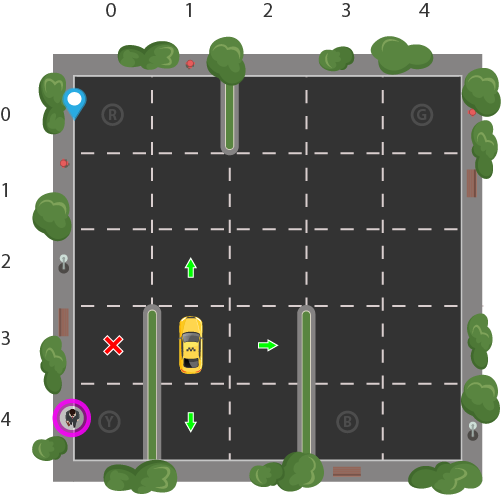
\includegraphics[width=0.9\linewidth]{img/qlearning}
  \end{center}
\end{wrapfigure}

L'objectif de cette étude est d'apprendre à une intelligence articifielle à  choisir le chemin optimal afin de:
\begin{itemize}
 \item récupérer les passagers et les déposer à leur destination,
 \item conduire en toute sécurité, ce qui signifie pas d'accidents,
 \item les conduire dans les plus brefs délais.
\end{itemize}

Nous utiliserons un environnement d'OpenAI Gym (Taxi-v3).

Un état est définit par \verb?(taxi_row, taxi_col, passenger_location, destination)?. Il y en a 25x5x4=500 et celui de l'image est (3,1,0,2), avec :
\verb?Passenger locations={0:'R(ed)',1:'G(reen)',2:'Y(ellow)',3:'B(lue)',4:'in taxi'}?
\verb?Destinations={0:'R(ed)',1:'G(reen)',2:'Y(ellow)',3:'B(lue)'}?
\verb?Actions={0:'move south',1:'move north',2:'move east',3:'move west',?
\verb?            4:'pickup passenger',5:'drop off passenger'}?

\end{frame}

\begin{frame}[fragile]
\frametitle{Application au Q-Learning (Reinforcement)}

\begin{wrapfigure}{r}{0.3\textwidth}
\vspace{-1cm}
  \begin{center}
    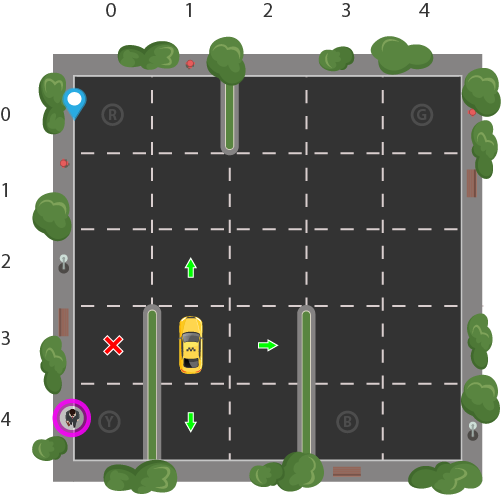
\includegraphics[width=0.9\linewidth]{img/qlearning}
  \end{center}
\end{wrapfigure}

Un état peut alors être représenté par un sommet d'un graphe, dont les arêtes sont pondérées, et les états accessibles par des états voisins. Les coefficients de pondération sont déterminés durant la phase d'apprentissage et sont utilisés dans la phase d'utilisation afin de guider les choix du taxi.

\begin{minipage}{0.35\linewidth}
\begin{tikzpicture}[scale=0.6]
\tikzstyle{sommetdec}=[]
\tikzstyle{arete}=[midway,fill=white]
\tikzstyle{sommet}=[circle,draw,fill=white,scale=0.6]
\node[sommet] (A) at (-0.5,0.5) {(3,1,0,2)};
\node[sommet] (B) at (-2,-1.5) {(2,1,0,2)};
\node[sommetdec] (C) at (-2,2.5) {};
\node[sommet] (D) at (1.5,2.5) {(4,1,0,2)};
\node[sommet] (E) at (1.5,-1.5) {(3,2,0,2)};
\node[sommetdec] (F) at (1.5,-4) {};
\node[sommetdec] (G) at (3,-1.5) {};
\node[sommetdec] (H) at (-4,-2.5) {};
\node[sommetdec] (I) at (-2,1.5) {};
\draw (A) -- (B) node[arete] {$0.6$};
\draw (A) -- (D) node[arete] {$0.3$};
\draw (A) -- (E) node[arete] {$0.1$};
\draw[dashed] (E) -- (F);
\draw[dashed] (C) -- (D) -- (G);
\draw[dashed] (I) -- (B) -- (H);
\end{tikzpicture}
\end{minipage}\hfill
\begin{minipage}{0.6\linewidth}
Un extrait de ce graphe montre que le meilleur choix dans cette configuration est d'aller à l'état (2,1,0,2) c'est à dire que la voiture doit monter.
\end{minipage}

\vspace{-0.2cm}
La simulation peut alors être effectuée grâce à un programme python.
\end{frame}

\begin{frame}[fragile]
\frametitle{Bibliographie}
\begin{itemize}
\item Ressource UPSTI Réforme des programmes 2021 - bases des graphes
\item Ressource UPSTI Réforme des programmes 2021 - parcours des graphes
\end{itemize}

\end{frame}

\end{document}
